%%% Chasopys Krayany
%%% ---------------
%%% PREAMBLE
%%% ---------------
\documentclass[10pt,a4paper]{article}

% Define geometry (without using the geometry package)
\setlength\topmargin{-48pt}
\setlength\headheight{20pt}
\setlength\headsep{0pt}
\setlength\marginparwidth{-20pt}
\setlength\textwidth{7.0in}
\setlength\textheight{10.0in}
\setlength\oddsidemargin{-30pt}
\setlength\evensidemargin{-30pt}

\frenchspacing						% better looking spacing

% Call packages we'll need
\usepackage[utf8]{inputenc}
\usepackage{CJKutf8}
\newenvironment{Japanese}{%
  \CJKfamily{min}%
  \CJKtilde
  \CJKnospace}{}
\usepackage[english,ukrainian]{babel}			% languages
\usepackage{graphicx}				% images
\usepackage{amssymb,amsmath}		% math
\usepackage{multicol}				% three-column layout
\usepackage{url}					% clickable links
\usepackage{marvosym}				% symbols
\usepackage{wrapfig}				% wrapping text around figures
\usepackage[T1,T2A]{fontenc}			% font encoding
\usepackage{charter} 				% Charter font for main content
\usepackage{blindtext}				% dummy text
\usepackage{datetime}				% custom date
	\newdateformat{mydate}{\monthname[\THEMONTH] \THEYEAR}
\usepackage[pdfpagemode=FullScreen,
			colorlinks=false]{hyperref}	% links and pdf behaviour

\makeatletter\chardef\l@japanese=255 \makeatother

% Customize (header and) footer
\usepackage{fancyhdr}
\pagestyle{fancy}
\lfoot{	\footnotesize 
Спільнота українців Японії ''Краяни'' / 
\begin{CJK}{UTF8}{}
\begin{Japanese}
在日ウクライナ人コミュニティ「クラヤニイ」
\end{Japanese}
\end{CJK}
\\
		\Mundus\ \href{https://www.facebook.com/ukrainians.japan}{www.facebook.com/ukrainians.japan}	\quad
	  }
\cfoot{}
\rfoot{\footnotesize ~\\ Сторінка \thepage}
\renewcommand{\headrulewidth}{0.0pt}	% no bar on top of page
\renewcommand{\footrulewidth}{0.4pt}	% bar on bottom of page

%%% ---------------
%%% DEFINITIONS
%%% ---------------

% Define separators
\newcommand{\HorRule}[1]{\noindent\rule{\linewidth}{#1}} % Creating a horizontal rule
\newcommand{\SepRule}{\noindent							 % Creating a separator
						\begin{center}
							\rule{250pt}{1pt}
						\end{center}
						}						

% Define Title en News input
\newcommand{\Category}[1]{%
		\begin{center}	
			\Large \usefont{T2A}{kurier}{m}{n}
			\underline{#1}%
		\end{center}	
		\par \normalsize \normalfont}
		
\newcommand{\JournalIssue}[1]{%
		\hfill \textsc{\mydate \today, Випуск №2}
		\par \normalsize \normalfont}

\newcommand{\NewsItem}[1]{%
		\usefont{T2A}{iwona}{m}{n} 
		\large #1 \vspace{4pt}
		\par \normalsize \normalfont}
		
\newcommand{\NewsAuthor}[1]{%
			\hfill \textsc{#1} \vspace{4pt}
			\par \normalfont}		

%%% ---------------
%%% BEGIN DOCUMENT
%%% ---------------
\begin{document}
% Title	
% -----
\JournalIssue{1}
		
\includegraphics[width=1\textwidth]{../common_files/chasopys_logo}
%\JournalName{Краяни - часопис українців Японії}
\noindent\HorRule{3pt} \\[-0.75\baselineskip]
\HorRule{1pt}
% -----

% Front article
\begin{center}
ВІТАЄМО З 25-Ю РІЧНИЦЕЮ НЕЗАЛЕЖНОСТІ УКРАЇНИ !
\end{center}

\SepRule

\vspace{0.1cm}

\begin{center}
\NewsItem{З Україною в серці - фестиваль ``День України`` 2016}	
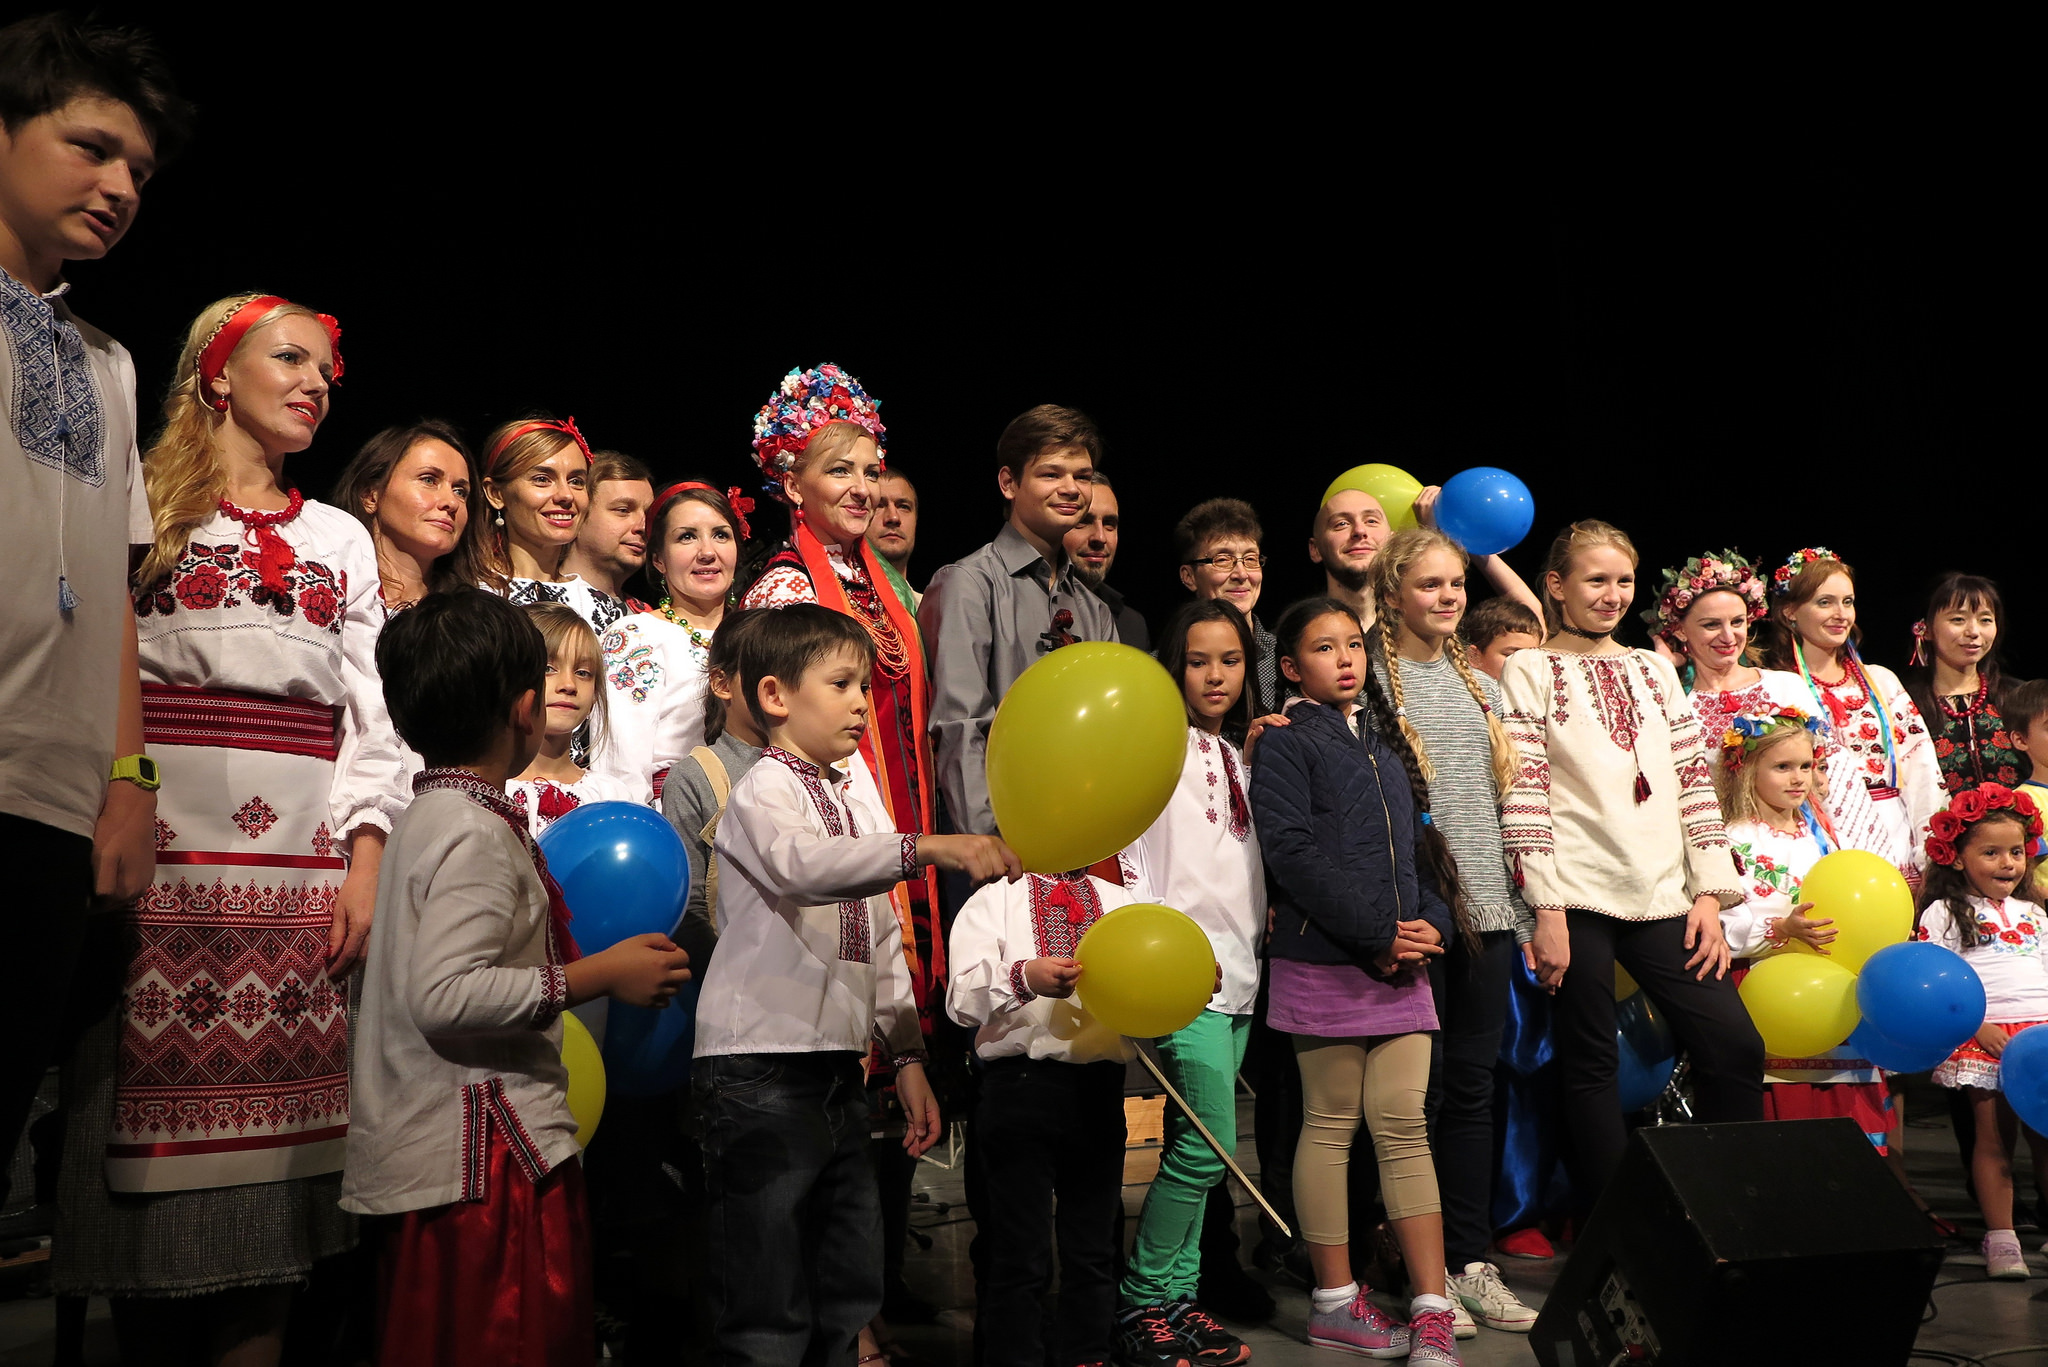
\includegraphics[width=0.8\textwidth]{images/18}
\end{center}
\SepRule	
\begin{multicols}{3}
В Токіо 20 листопада відбувся щорічний український фестиваль ``День України``, який цього року носив назву ``З Україною в серці`` kraiany.github.io/festival В рамках фестивалю пройшли численні виставки, майстер-класи та презентації українських об'єднань в Японії. О 15 годині розпочалась урочиста концертна програма за участі як українців, які проживають в Японії, так і гостей, які прибули з України. Режисером-постановником заходу була Вікторія Верескун. Зі струн тріо молодих скрипалів Іллі Бондаренка та Тетяни Жмендак Two Violins та фортепіанного супроводу Наталі Лебедєвої прозвучали твори програми ``Бах у джазі``. Своїм виконанням музиканти відкривають ці витвори мистецтва Пінзеля для всього світу. Сопрано, відома співачка японської опери, народна артистка України Оксана Степанюк приєдналась до заходу з виконанням українських пісень. Вихованці української школи в м.Токіо Школа Джерельце запалили своєю енергією весь зал активними танцями та театральними постановками. Українські народні та сучасні хореографічні композиції, народні пісні прозвучали у виконанні професійних та аматорських виконавців з Токіо. Цього року до організації заходу долучилось Посольство України в Японії, сприявши проведенню заходу у концертній залі громадського центру одного з центральних районів Токіо - Мінато-ку.
\end{multicols}

\newpage

\Category{2015 рік}

\begin{multicols}{3}

\NewsItem{Лялька-мотанка}
\NewsAuthor{Йокогама}
\begin{center}
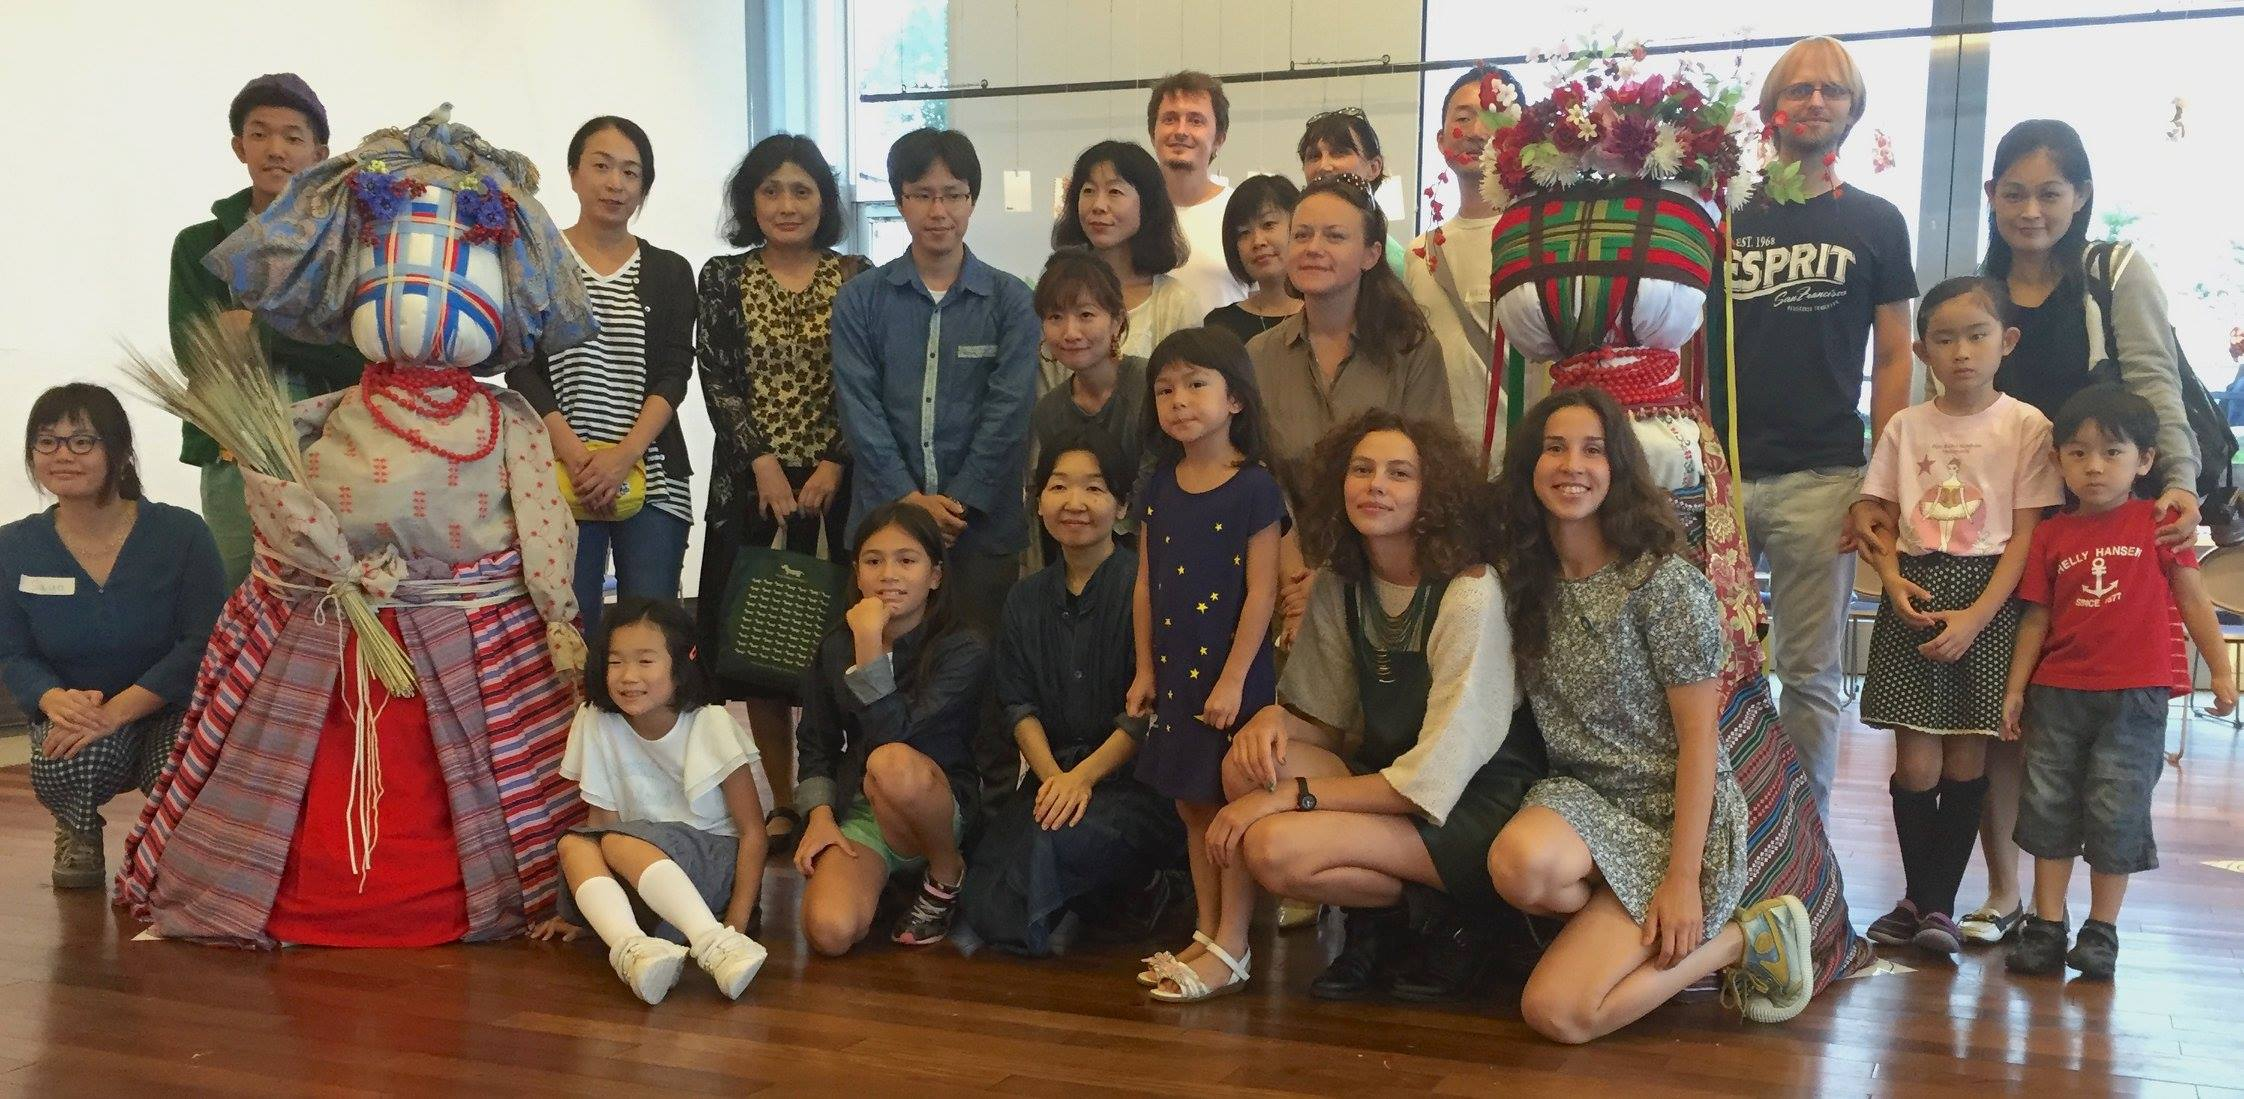
\includegraphics[width=0.8\linewidth]{images/1}
\end{center}
26 вересня відбулася чудова мистецька акція. В Йокогамському припортовому парку ``Зоо-но-хана`` (парк Хобота Слона – названий так, бо невеликий півострів, на якому розташований парк, справді нагадує формою хобіт) — українська художниця Олена (Leka) Дерев’янкіна (facebook.com/artist.leka) організувала і провела майстер-клас та одночасну артистичну інсталяцію. Разом з учасниками, відвідувачами кафе — дітьми та дорослими, японцями, українцями та гостями з інших країн — було ``збудовано`` дві великих, майже в людський зріст, ляльки-мотанки. Через розмір ляльок, клаптиками тканини було важко обійтися, тож на виготовлення ляльок пішли ящики старого одягу, кілька клубків ниток, відрізи тканини на плахти лялькам-``дівчатам``, квіти та стрічки для віночка ``молодшій`` з них, та ще й сніп жита старшій ``заміжній`` мотанці. Діти та дорослі також робили аплікації на поштових листівках, які пізніше будуть відіслані в дитячі будинки України. А малюки з задоволенням дивилися відеопрограму з мультиками про козаків та українською тематичною підбіркою відео. Дякуємо Олені за чудову організацію заходу, гарний настрій і прекрасно проведений час.

\vspace{1cm}

\NewsItem{Урок української вишивки}
\NewsAuthor{Йокогама}
\begin{center}
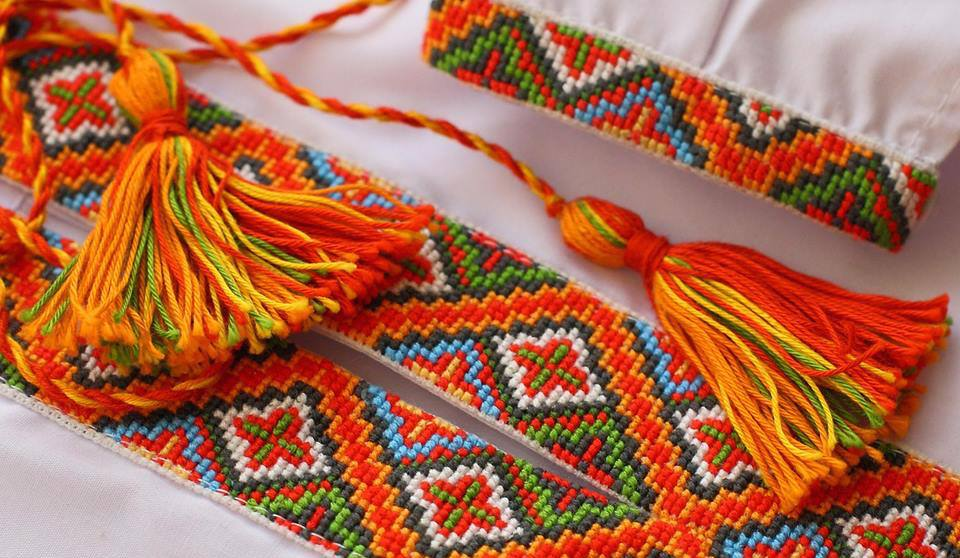
\includegraphics[width=0.8\linewidth]{images/2}
\end{center}
30 вересня в Йокогамі Ірина Вєтрова провела пробний урок з вишивання. В майбутньому курсом передбачений екскурс в історію української вишивки та значення символіки, навчання типів українських швів виготовляючи різні вироби, починаючи від прикрас і поступово переходячи до більш складних речей. 

\vspace{1cm}

\NewsItem{Перше Богослужіння о.Йвана}
\NewsAuthor{Токіо}
\begin{center}
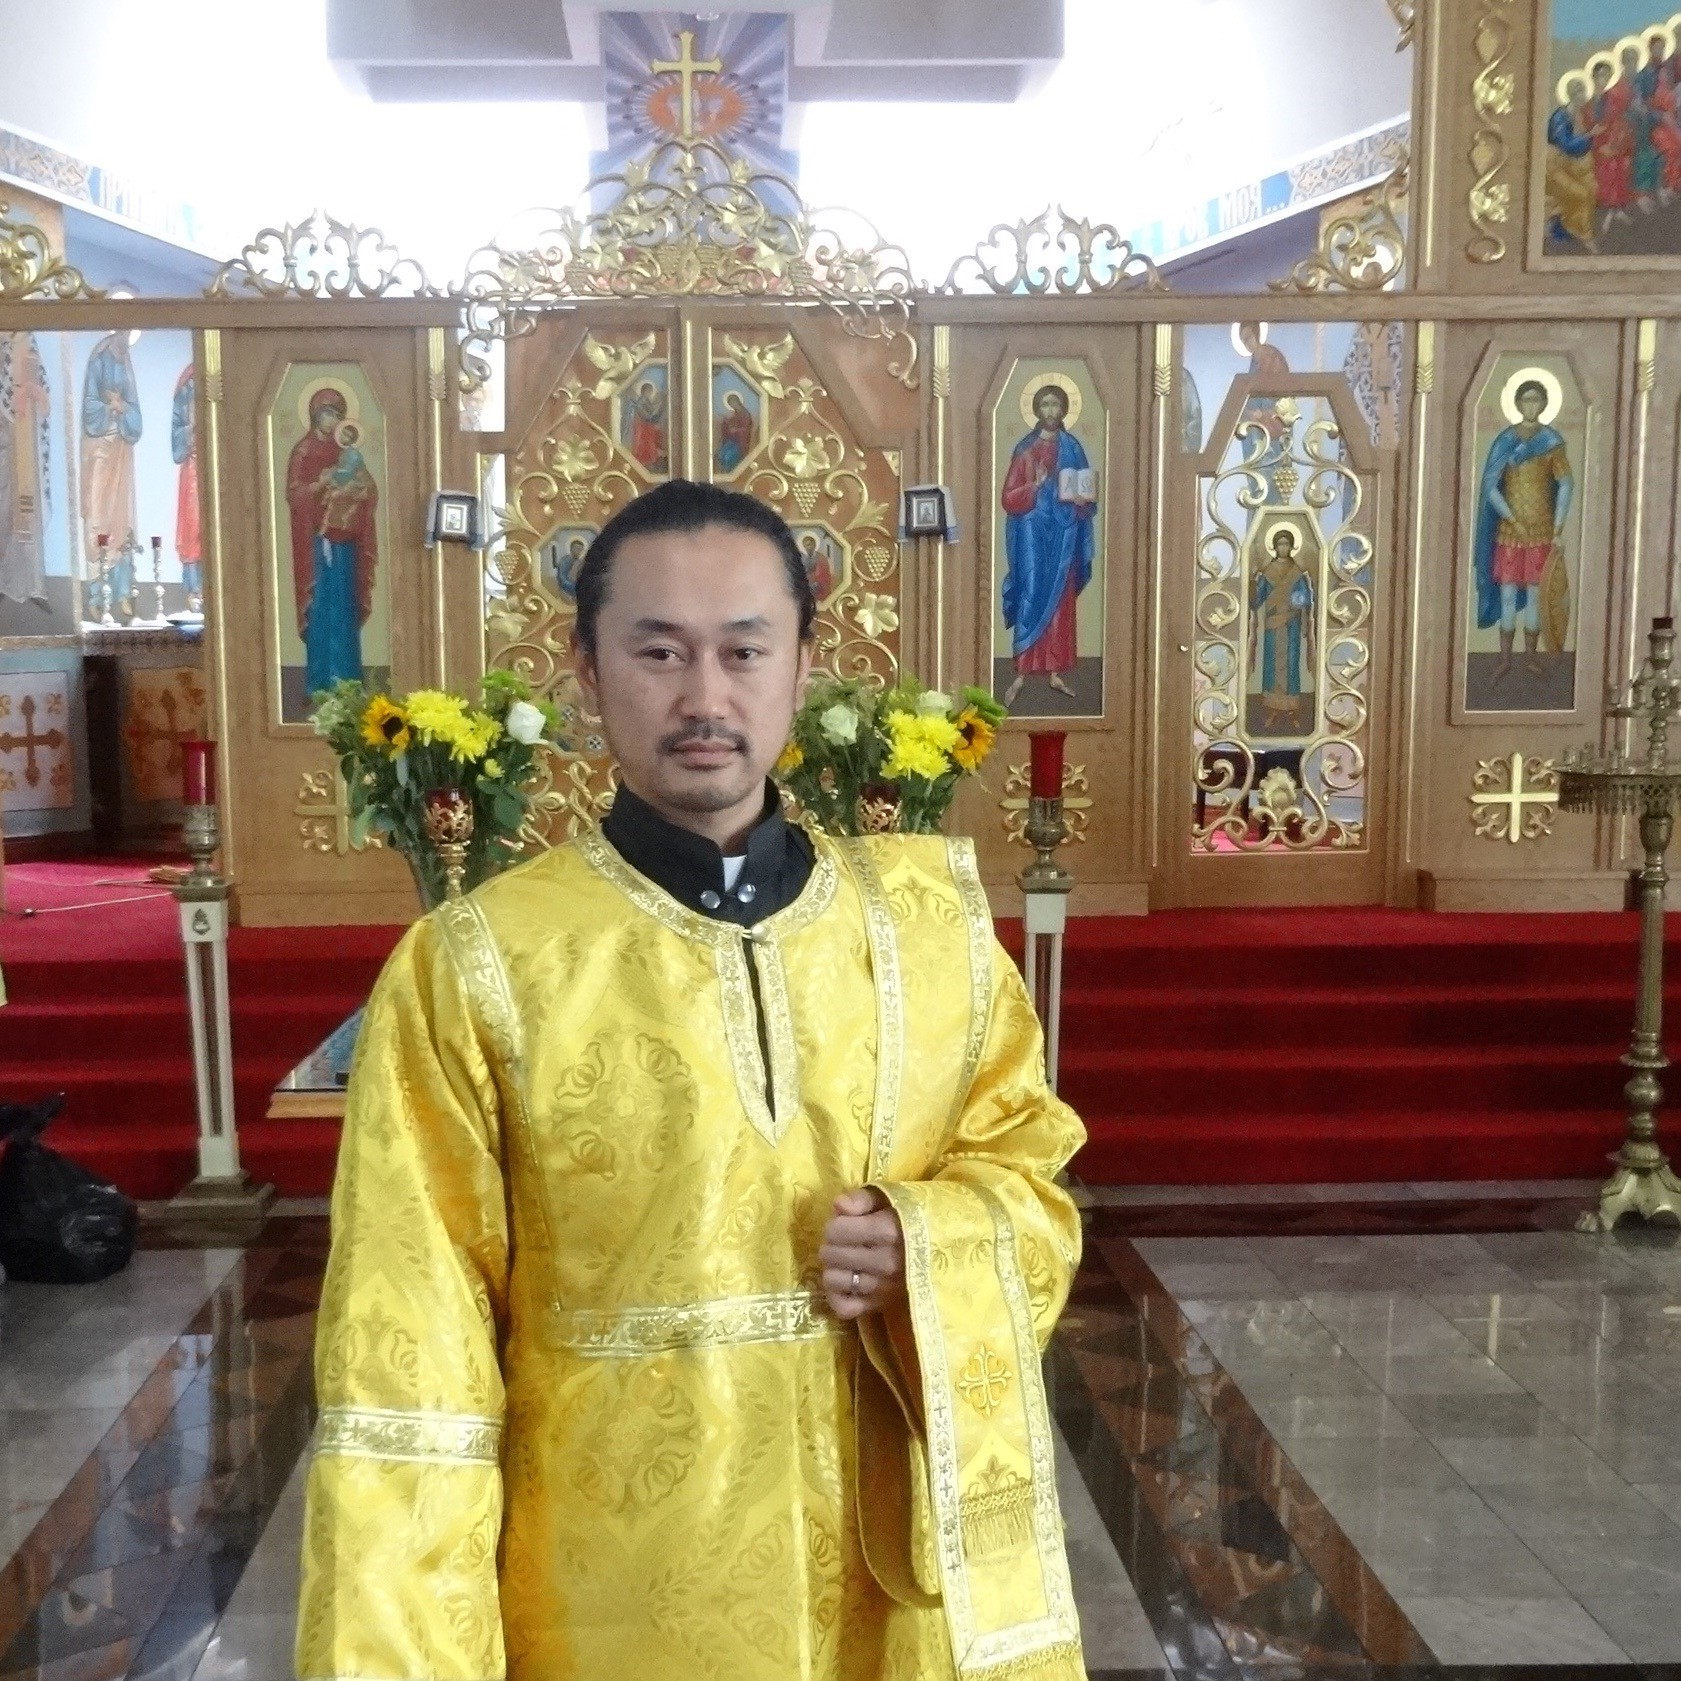
\includegraphics[width=0.8\linewidth]{images/3}
\end{center}
В місії Української Церкви Київського Патріархату в Токіо 4 жовтня Богослужіння провів отець Йван. Це була його перша служба в Японії як диякона. Бажаємо о.Йвану многая літа! За традицією після літургії відбувся спільний обід вірян.

\vspace{1cm}

\NewsItem{Поминальна Служба з вшанування пам'яті жертв Голодомору}
\NewsAuthor{Токіо}
\begin{center}
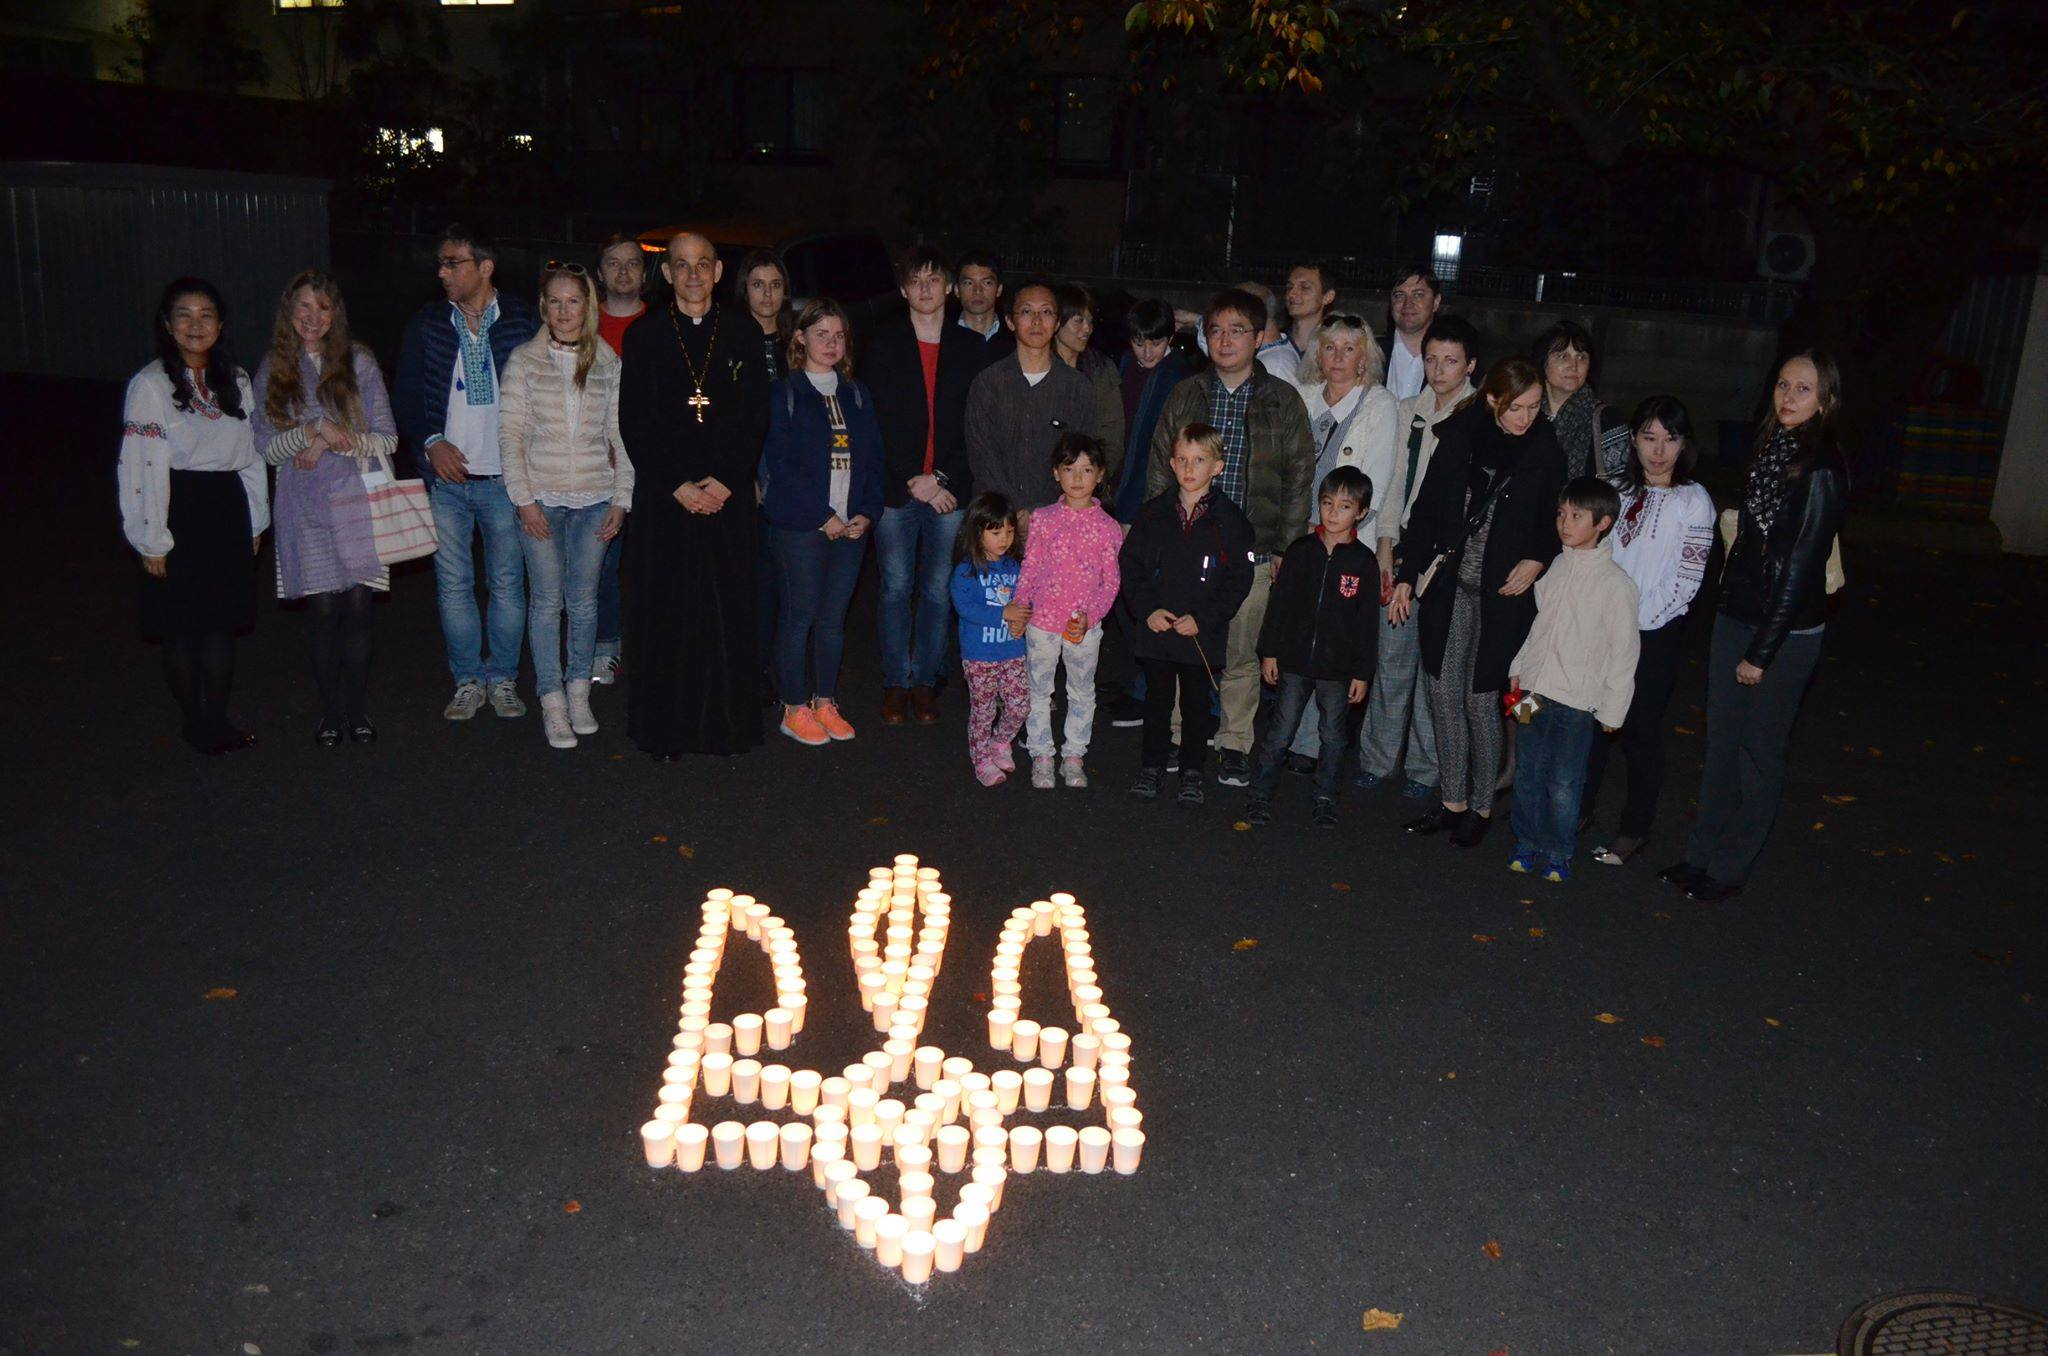
\includegraphics[width=0.8\linewidth]{images/4}
\end{center}
Місія Української Православної Церкви Київського Патріархату провела поминальну службу в пам'ять жертв Голодомору 1932-1933 років. Серед близько 50 учасників дійства були громадяни Японії, України, США, Канади та Німеччини. За ініціативи активістів громади українців в Японії ``Краяни`` після молебню за жертвами ХХ століття та Героями сьогодення учасники виклали зі свічок тризуб та прочитали молитву. Панахида за упокій душ жертв геноциду була проведена на прохання Надзвичайного та Поважного Посла України в Японії Ігоря Харченка, який відвідав захід з офіційним візитом.

\vspace{1cm}

\NewsItem{Другий український фестиваль реґіону Канто - Український День}
\NewsAuthor{Йокогама}
\begin{center}
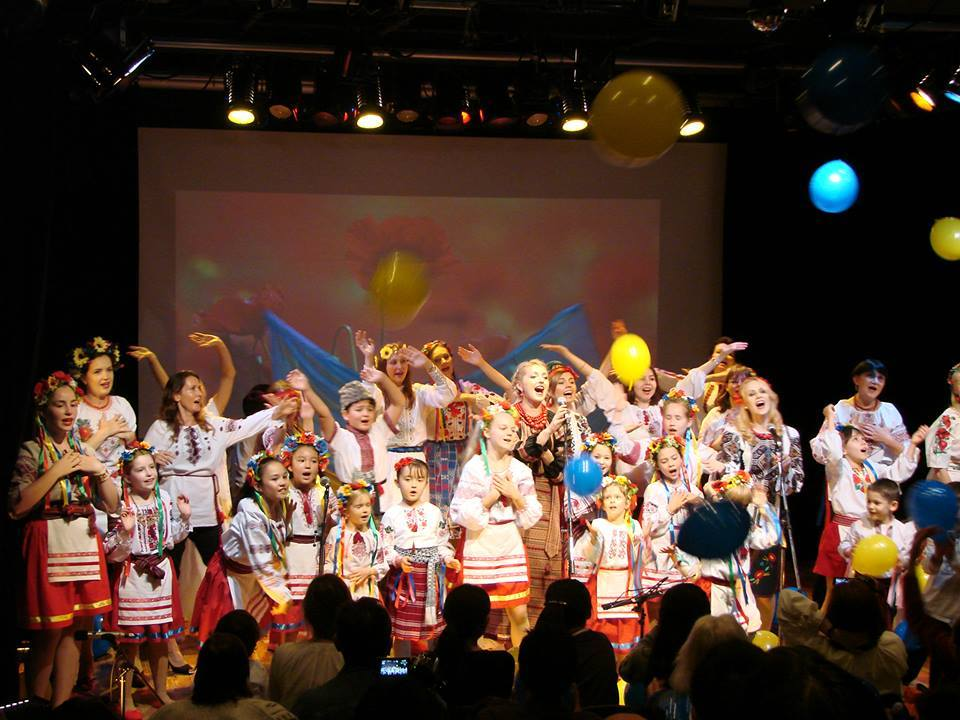
\includegraphics[width=0.8\linewidth]{images/5}
\end{center}
15 листопада в Шін Йокогамі успішно пройшов Другий український фестиваль реґіону Канто - Український День. Гості фестивалю знайомились з українськими традиціями, роботaми українських майстрів. Працював ресторан, де бажаючі змогли скуштувати українських страв, солодощі і українські вина. Проводились різноманітні майстер класи, де гості власноруч виготовляли писанки, мотанки, листівки з вибійкою. На завершення гостей порадували своїми виступами професійні актори і співаки, аматори та дитячий колектив української, школи Джерельце, що в Токіo. Захід організувала громада українців в Японії ''Краяни'' за підтримки Посольства України в Японії та St. Jude Ukrainian Orthodox Mission, Tokyo. Головним спонсором фестивалю були оргкомітет ''Український день'' та студія ''Альта'', де і відбувся фестиваль. Виручені на фестивалі кошти (близько 2000 доларів США) були передані на допомогу потерпілим від війни в Україні.

\end{multicols}

\newpage

\begin{multicols}{3}

\NewsItem{У Японії продають ``Самурайські пісні`` для допомоги пораненим в АТО}
%\NewsAuthor{Йокогама}
\begin{center}
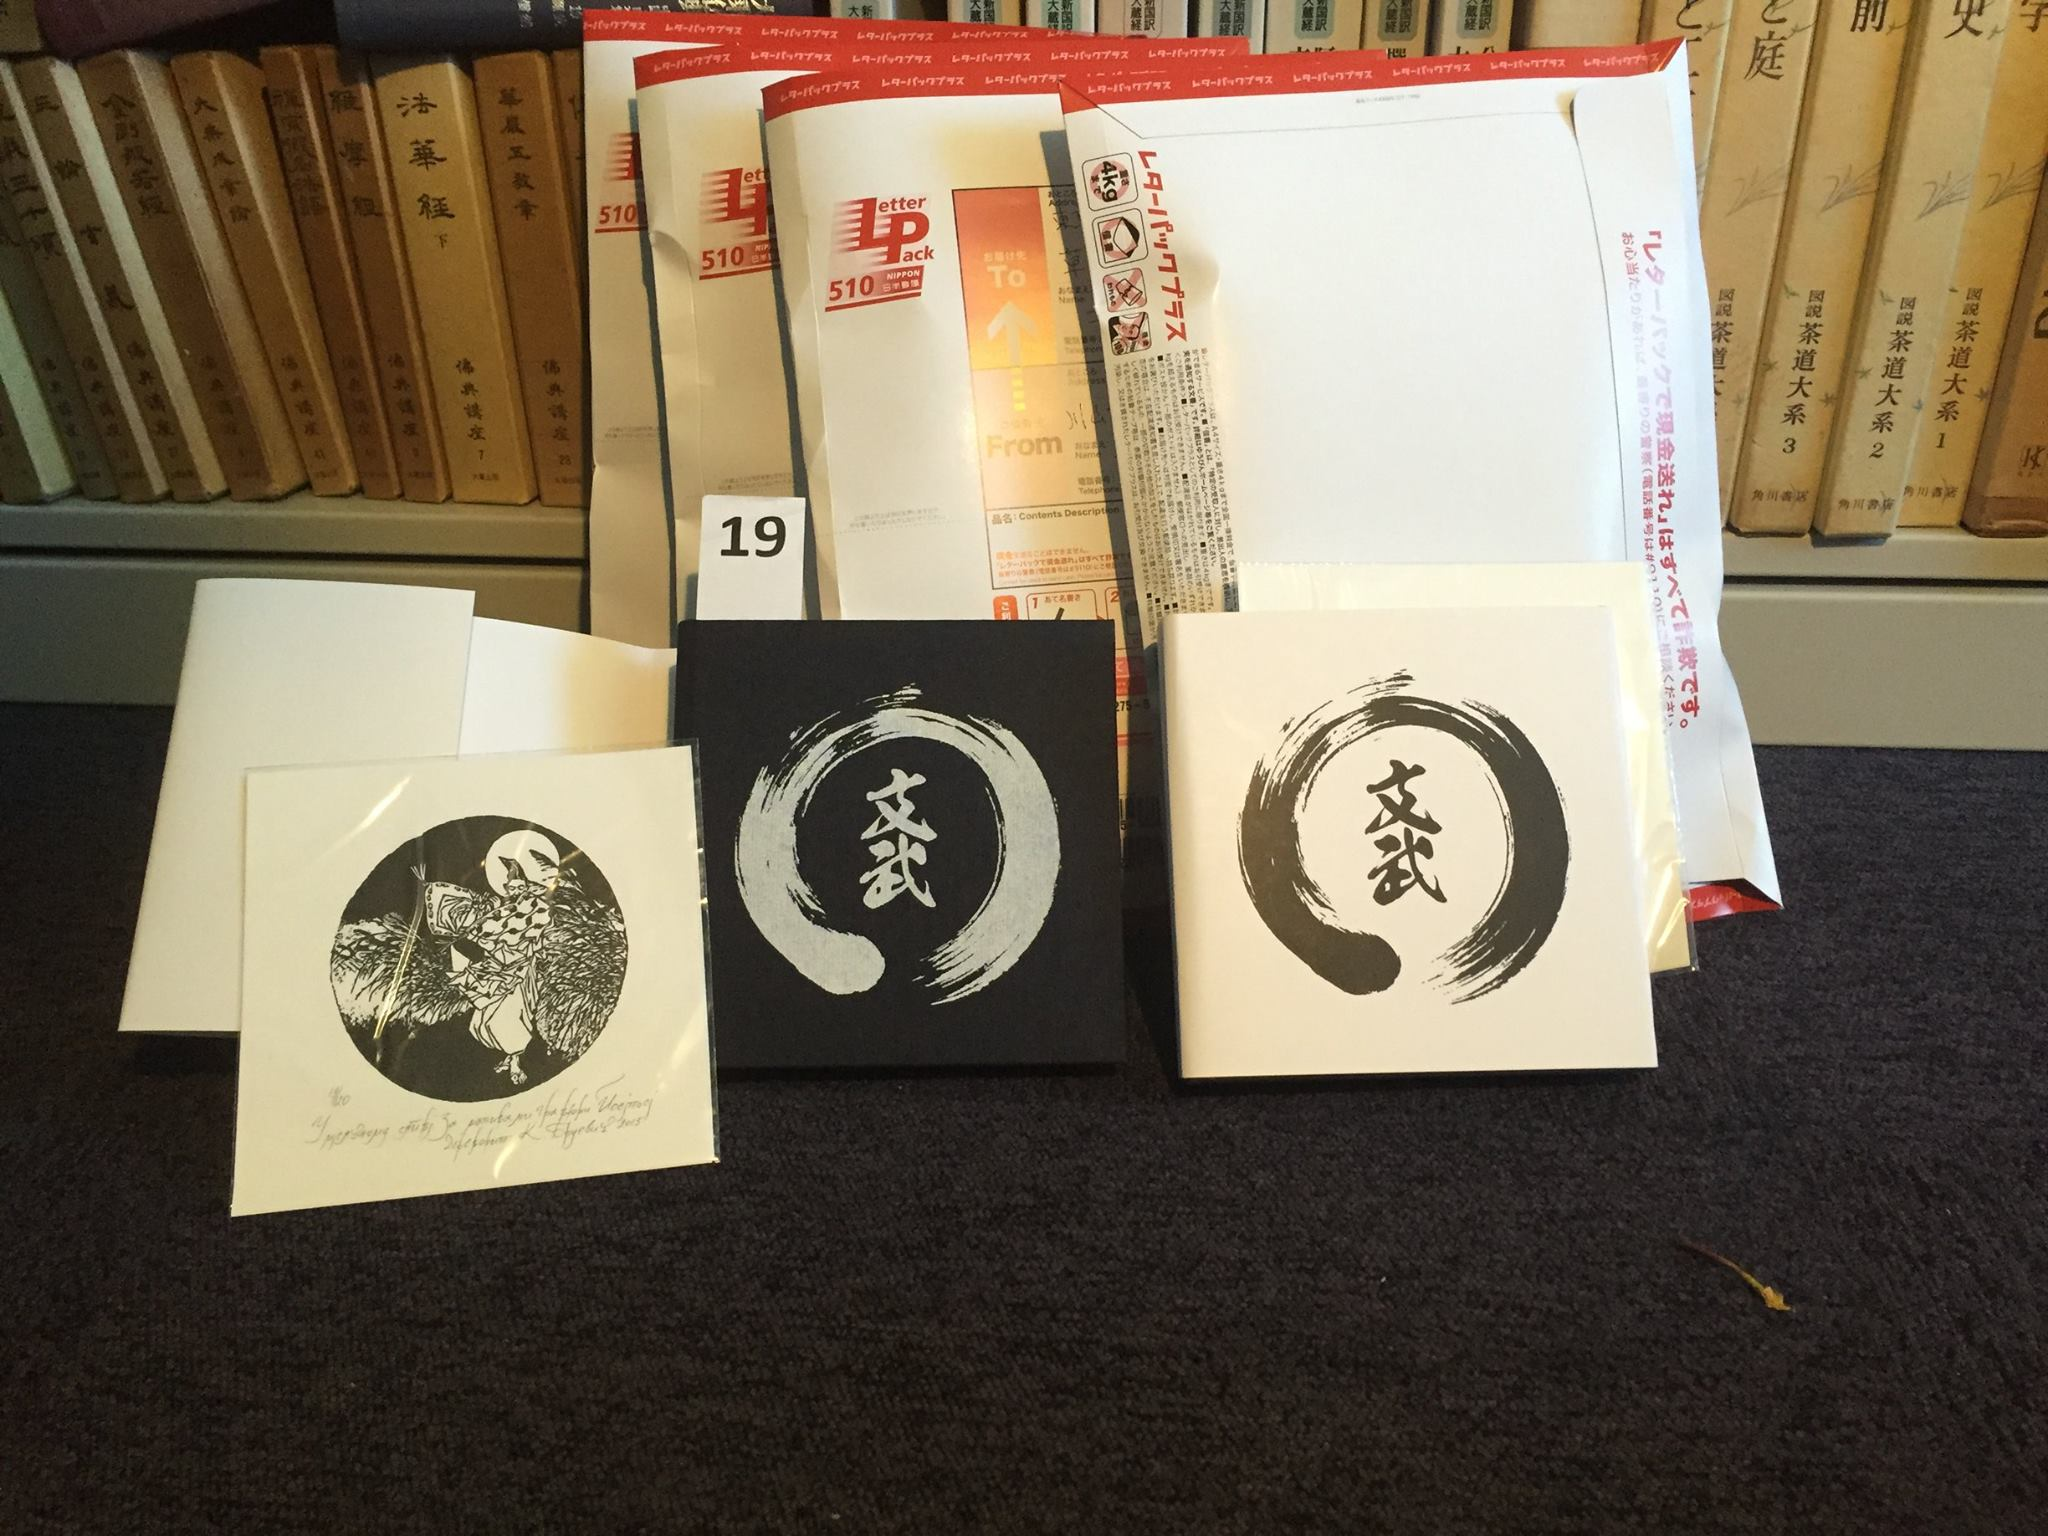
\includegraphics[width=0.8\linewidth]{images/6}
\end{center}
Спільнота українців у Японії оголосила збір пожертв на лікування поранених бійців. Натомість пропонують примірник книги ``Самурайські пісні`` в українському перекладі. У спільноті українців у Японії ``Краяни`` в соцмережі зазначають, що книгу можна отримати за пожертву в 10 тис. ієн, це близько 200 грн. Всі зібрані кошти перерахують на біотех-реабілітацію пораненим. ``Це унікальна збірка перекладів на українську мову самурайської поезії з коментарями та післямовою. Лімітований тираж у 111 примірників. 270 сторінок у твердій обкладинці. Ілюстроване видання у дзенському стилі. До кожного примірника додається справжня гравюра ``У місячному сяйві`` українського митця Катерини Бруєвич. Найкращий подарунок пораненим хлопцям та вам особисто на Новий рік``, - пишуть в оголошенні. Автор книги Андрій Накорчевський - професор японського Університету Кейо в Токіо. З самого початку він замислював видання ``Самурайських пісень`` як благочинний проект для збору коштів пораненим у АТО.

\vspace{2cm}

\NewsItem{Житомирянка в Японії готує українські страви для відвідувачів ресторанів}
\NewsAuthor{Токай}
\begin{center}
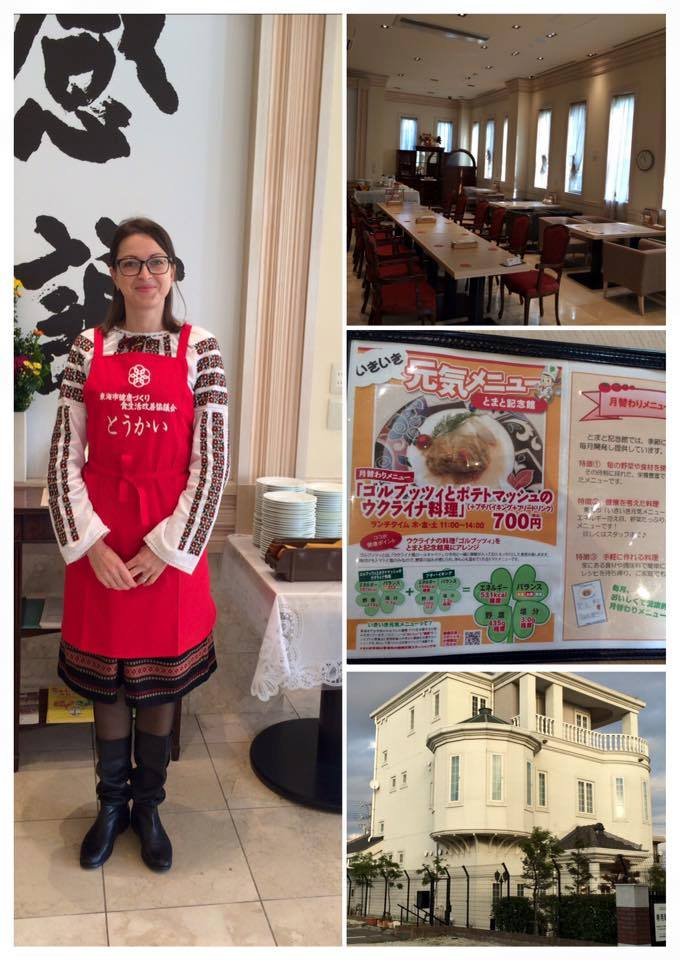
\includegraphics[width=0.8\linewidth]{images/7}
\end{center}
Протягом грудня відвідувачів ресторану ``Ада-Кода`` та ресторану в Будинку томатів в японському місті Токай, пригощали українськими стравами. Місячник української кухні проходив за підтримки місцевої влади. Шеф-кухар Людмила Кавагучі розповідає, що у меню увійшли голубці, картопляне пюре, холодець, салат з капусти і кропу, борщ з пампушками та вареники з картоплею і шкварками. ``Працюю над українськими обідами для місцевих ресторанів. Найбільше японцям сподобалися голубці та салат з капусти і кропу, - розповідає українка. - Холодець пішов на ``ура``. В японській кухні є схожа страва - нікогорі. Тільки у них замість свинини - креветки, морські їжаки та інші морепродукти``. Готувати українські страви Людмила навчилася у рідному Житомирі. П'ять років тому вийшла заміж за японця і переїхала до Японії. ``Намагаюсь популяризувати Україну. В Японії проблематично знайти деякі продукти для українських страв. Буряк дуже складно купити, кріп доводиться замовляти з України``.

\vspace{1cm}

\NewsItem{У Японії будинок-музей перетворили на український Різдвяний дім}
\NewsAuthor{Йокогама}
\begin{center}
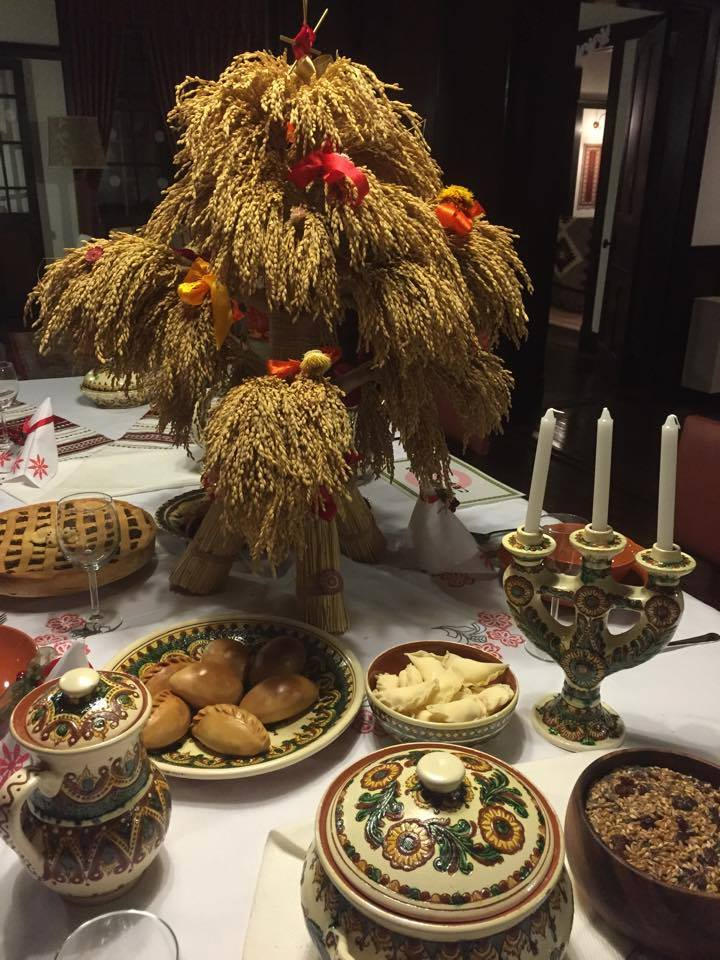
\includegraphics[width=0.8\linewidth]{images/9}
\end{center}
У Будинку дипломатів японського міста Йокогама триває експозиція ``Українське Різдво``. А на свято Миколая, 19 грудня, учні української школи заспівали там різдвяних пісень. Про це повідомляє VIDIA з посиланням на спільноту Українців в Японії ``Краяни``. Впродовж 16 років зимова Йокогама знайомить японців і гостей з традиціями святкування Різдва в різних країнах світу. Цього року разом з Британією, Канадою, Францією, Австрією, Австралією та Німеччиною вперше представлена Україна. Три тижні в сторічному будинку вікторіанського стилю буде панувати затишок сімейного Українського Різдва. У рамках українського Різдвяного дому відбулись майстер класи з плетіння Різдвяного павука та писанкарства.

\end{multicols}

\newpage

\Category{2016 рік}

\begin{multicols}{2}

\NewsItem{Акція на підтримку Надії Савченко}
\NewsAuthor{Токіо}
\begin{center}
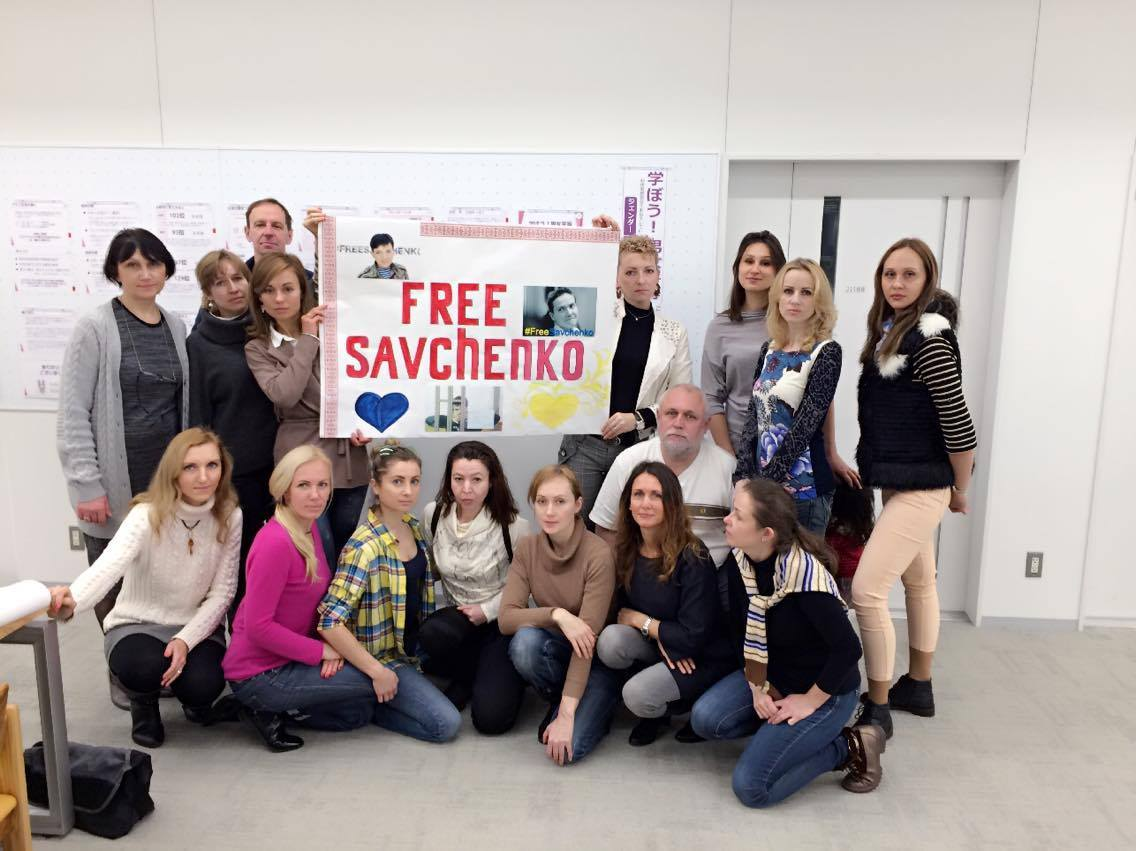
\includegraphics[width=0.8\linewidth]{images/12}
\end{center}
Українці в Японії приєдналися до акції ``День глобальної підтримки Free Savchenko``. Вони виготовили плакат із зображенням української льотчиці і написом ``Свободу Савченко`` і сфотографувалися з ним. Крім того українське посольство змінило свою обкладинку в соціальній мережі на фотографію Савченко. Нагадаємо, міністр закордонних справ України Павло Клімкін закликав світову спільноту підтримати акції на захист утримуваної в російському СІЗО української льотчиці, народного депутата Надії Савченко.

\vspace{1cm}

\NewsItem{Зустріч Президента з українською громадою Японії}
\NewsAuthor{Токіо}
\begin{center}
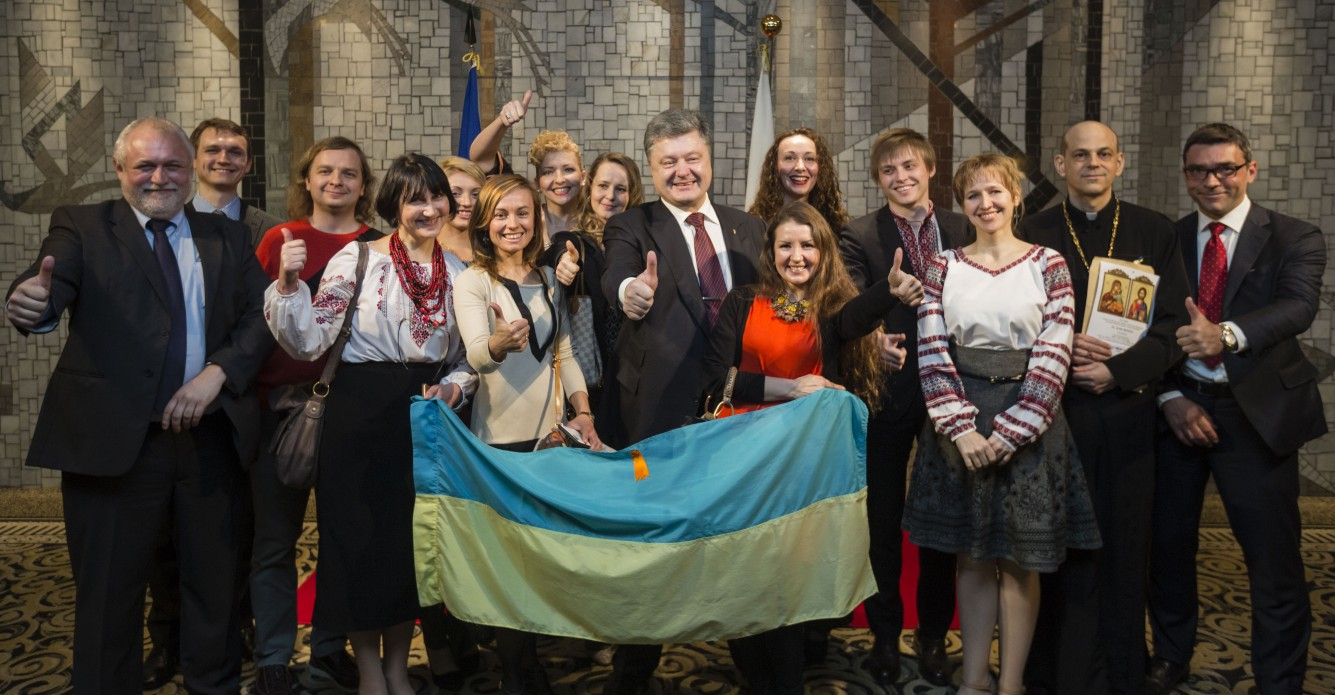
\includegraphics[width=0.8\linewidth]{images/13}
\end{center}
Президент України Петро Порошенко зустрівся з українською громадою в Токіо, перебуваючи в Японії з офіційним візитом. ``Я радий нагоді зустрітися з моїми співвітчизниками, які живуть, працюють та вчаться на японській землі``, - сказав Президент. ``Надважливою також є солідарність українських громадян``, - зазначив Президент, подякувавши, громаді українців ``Краяни`` за активну солідарну позицію з Батьківщиною. Глава держави подякував за небайдужість до долі України, зокрема відзначив фінансову та матеріальну допомогу українців в Японії для українських військових, які беруть участь в АТО, та внутрішньо-переміщених осіб з тимчасово окупованих територій. Президент ще раз наголосив, що 2017 рік буде роком Японії в Україні та запросив українську громаду долучитися до цієї акції. ``Приємно усвідомлювати, що, незважаючи на велику відстань, ви не втрачаєте свого українського коріння, своєї ідентичності``, - наголосив Петро Порошенко звертаючись до українців Японії. Глава держави переконаний, що кожен українець в Японії продовжує вболівати за долю нашої держави. Президент розповів про результати домовленостей з японською владою і наголосив, що українсько-японські стосунки мають інтенсивний рівень. Глава держави також повідомив, про наміри української влади всіляко стимулювати вивчення японської мови в Україні та активізувати обмін між студентами задля зближення двох країн, культурного та наукового обміну.

\vspace{1cm}

\NewsItem{Українську бандуристку Наталю Гудзій нагородили почесною грамотою МЗС Японії}
%\NewsAuthor{}
\begin{center}
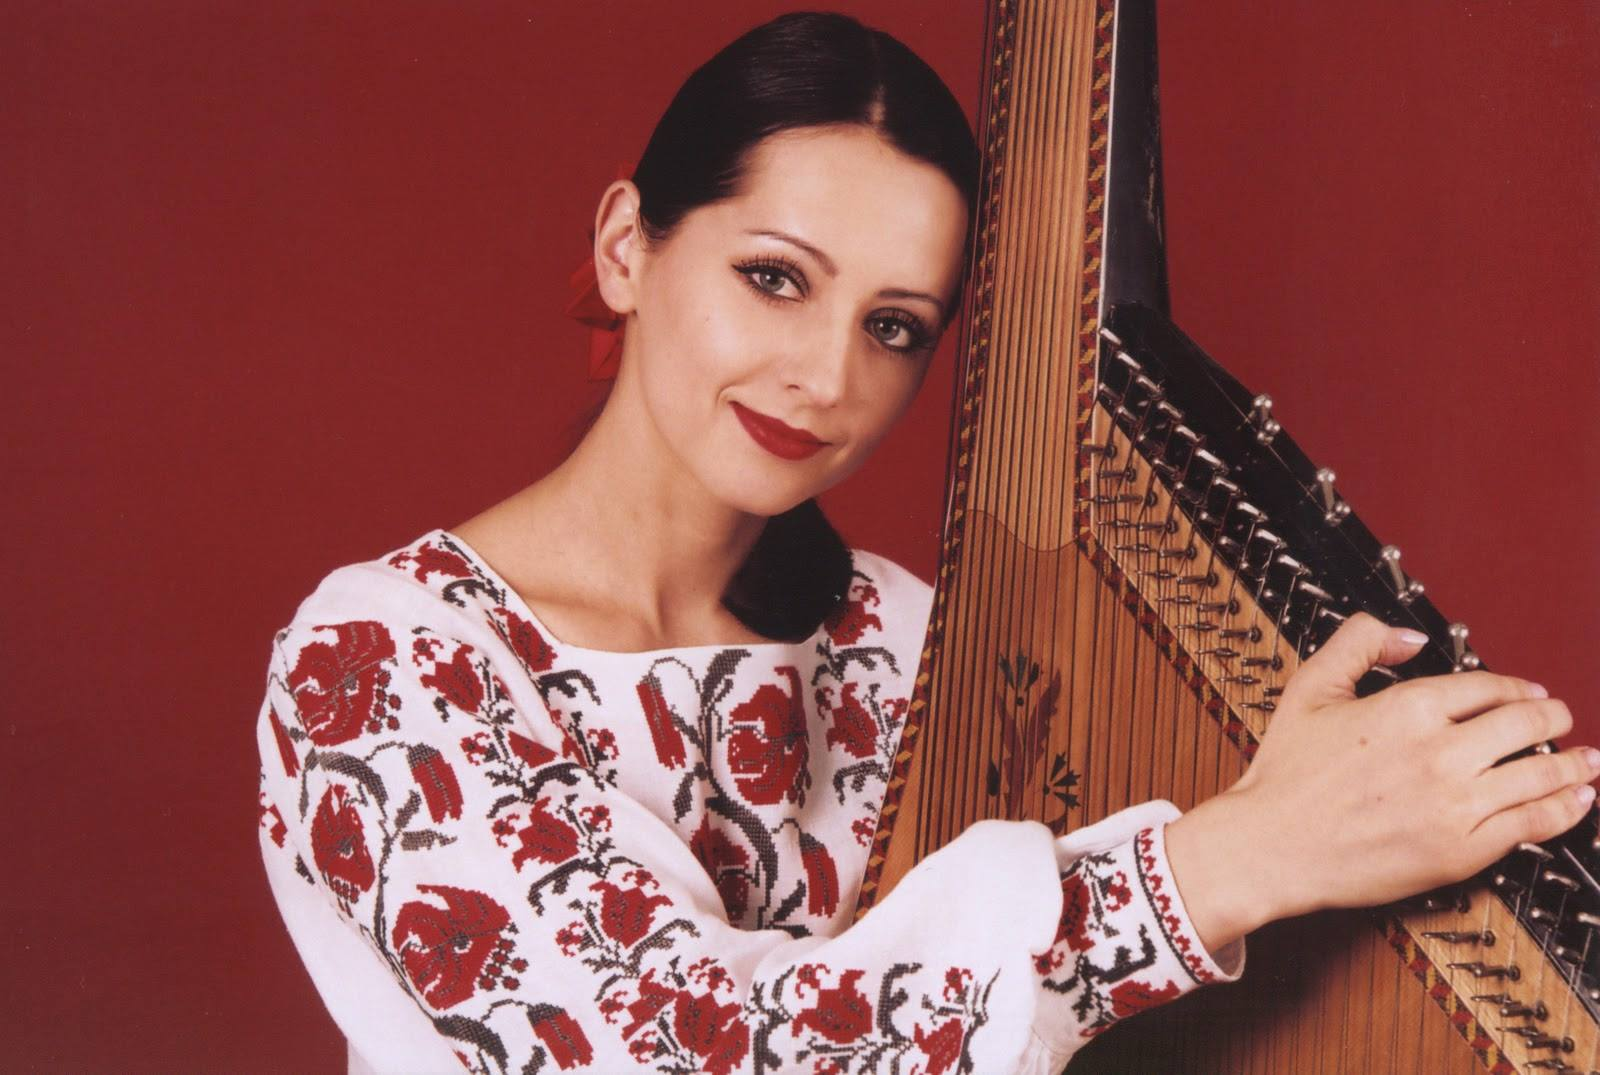
\includegraphics[width=0.8\linewidth]{images/15}
\end{center}
Кожного року Міністерство закордонних справ Японії нагороджує почесними грамотами осіб та організації, які досягли значних успіхів у своїй діяльності, відзначаючи їх внесок у розвиток дружніх відносин між Японією та багатьма іншими країнами, а також внесок у мир та стабільність в Японії та усьому світі. У 2016 році почесними грамотами буде нагороджено 142 осіб та 31 організацію. Серед них пані Наталія Гудзій (особиста нагорода), українська співачка та бандуристка, яка народилася в Україні, але упродовж тривалого часу живе та веде активну діяльність в Японії. Щиро вітаємо пані Наталю та бажаємо нових творчих здобутків!

\end{multicols}

\newpage

\begin{multicols}{2}

\NewsItem{В місті Нагоя пройшов мегамарш у вишиванках}
\NewsAuthor{Нагоя}
\begin{center}
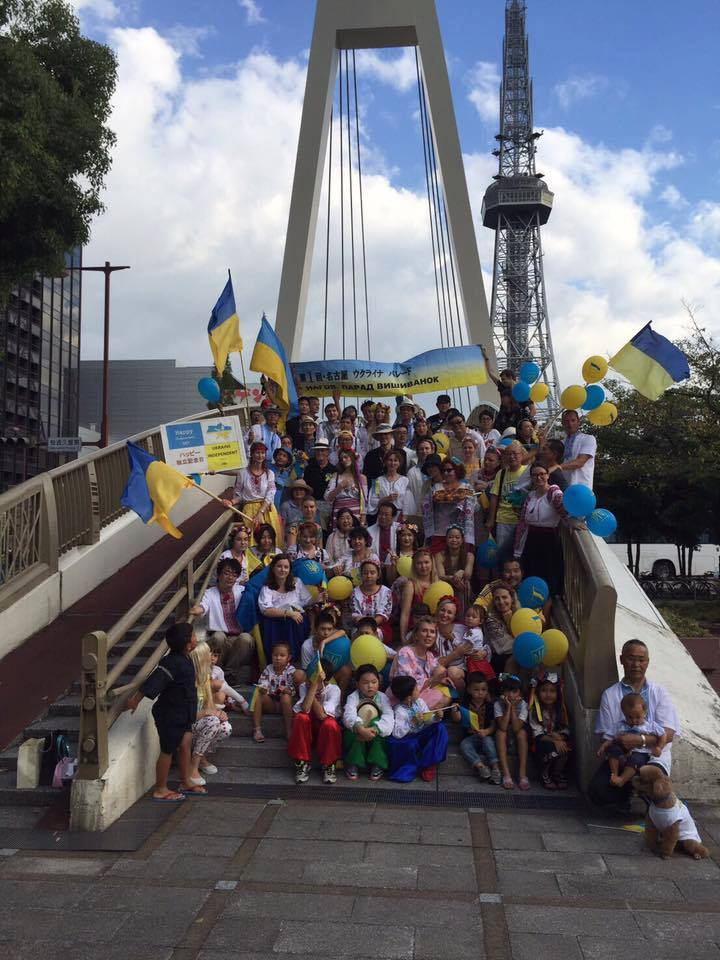
\includegraphics[width=0.8\linewidth]{images/16}
\end{center}
В одному з найбільших міст Японії - Наґої - українці влаштували урочистий мегамарш у вишиванках, присвячений 25-й річниці незалежності України. Як повідомила спільнота Українці в Японії Краяни, мегамарш пройшов у суботу, 3 вересня. ``Українці та близькі за духом друзі України третього вересня зібрались на першому українському параді в місті Наґоя, що є четвертим за кількістю мешканців містом Японії``, - йдеться в повідомленні. Зазначається, що особливим символом параду був коровай, спечений переселенкою з окупованої Горлівки Донецької області. У марші вишиванок взяло участь близько 100 людей. Серед учасників ходи були як українці, так і японці, і навіть домашні улюбленці. Парад у вишиванках в Японії вперше відбувся в 2013 році у місті Токіо та став традиційним дійством для українців, японців та друзів України з інших країн. В 2016 році в Токіо відбувся 4-й мегамарш у вишиванках, відомий в Японії як Ukraine Parade.

\vspace{2cm}

\NewsItem{Візит Архієпископа Євстратія (Зорі) до Японії}
\NewsAuthor{Токіо}
\begin{center}
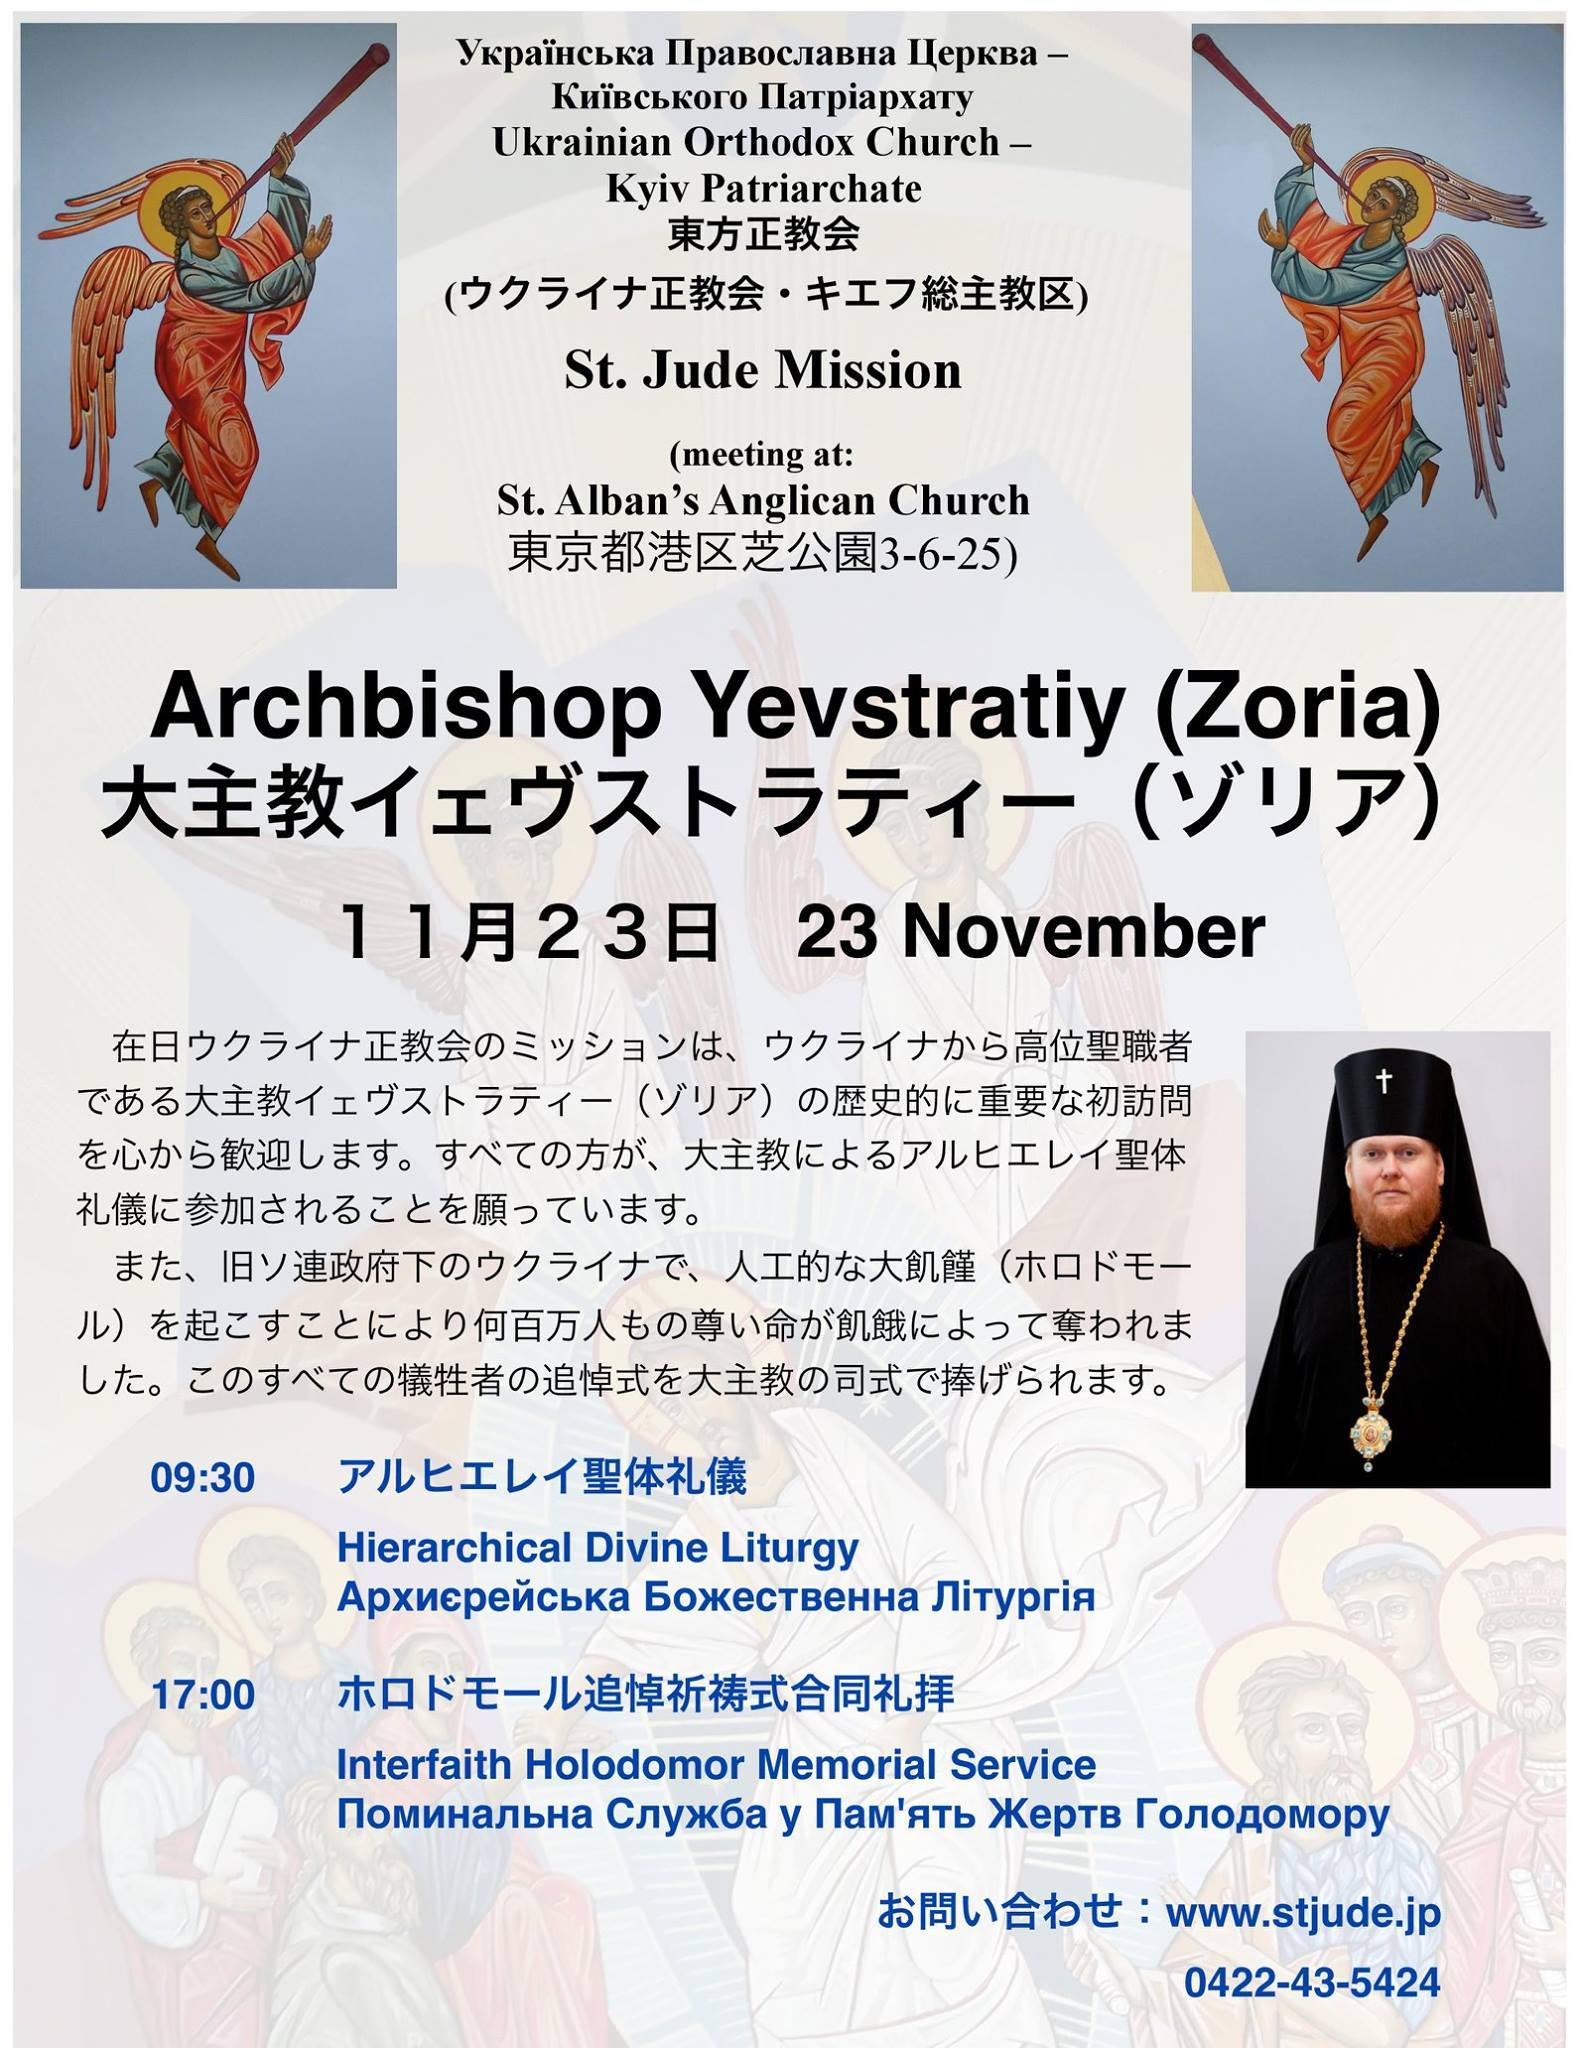
\includegraphics[width=0.8\linewidth]{images/19}
\end{center}
У листопаді відбулася важлива віха у житті громади Української Православної церкви Київського патріархату St. Jude Ukrainian Orthodox Mission, Tokyo - перший візит ієрарха з України Архієпископа Євстратія (Зорі). У середу 23 листопада о 9.30 відбулася Ієрархічна Божественна Літургія. До 83-ої річниці пам'яті Голодомору в Україні у 1932-33 роках на прохання Посла України в Японії Ігоря Харченка 23 листопада о 17 годині відбулася поминальна Служба. На літургію були запрошені представники усіх віросповідань. Молитви прочитали представники християнського (католицьке, протестантське, православне), єврейського та мусульманського духовенства.

\end{multicols}

\newpage

\Category{Розповіді з життя українців в Японії}

\begin{multicols}{3}

\NewsItem{Українці мають можливість навчатися в Японії. Історія вінничанина, який потрапив в Токіо}
\NewsAuthor{За матеріалами vn.20minut.ua}
\begin{center}
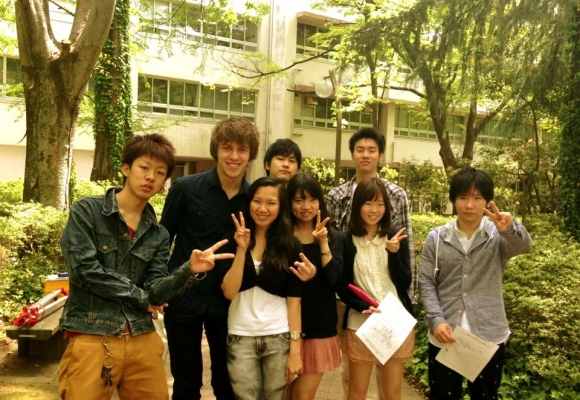
\includegraphics[width=0.8\linewidth]{images/10}
\end{center}
Вінничанин Максим Люльчук закінчив третій курс в Токійському Аграрному Університеті. Хлопець розповідає про особливості навчального процесу та життя українських студентів в Японії. Програма співпраці Токійського Аграрного Університету та Національного Університету Біоресурсів і Природокористування України (колишній Національний Аграрний Університет) в Києві тривала з 2004 по 2014 рік. Щороку, навесні один або двоє студентів НУБіП вирушали здобувати ступінь бакалавра в Токіо. Студентам надавалася щомісячна стипендія, приблизно еквівалентна 400 доларам США, безплатний гуртожиток та можливість працювати невелику кількість годин на тиждень.Взяти участь у відборі могли студенти будь-якого факультету НУБіП, але у Токіо вони всі мали навчатися лише на одному факультеті – Сільського господарства та харчової промисловості, за спеціальністю Міжнародний біо-бізнес.

Для того, щоб керівництво університету з усіх претендентів обрало саме тебе, потрібно було абсолютно вільно володіти англійською, як письмовою, так і усною, бути комунікативним та вмотивованим і вміти довести цю мотивацію відбірковій комісії, а також – бути готовим присвячувати багато часу вивченню японської і мати змогу оплатити собі квиток до Токіо. Максим був не першим вінничанином, який вирушив в Країну вранішнього сонця за даною програмою. З 2006 по 2012 у Токійському Аграрному університеті навчався інший вихідець з Вінниці – Сергій Леонтьєв. Після здобуття ступеню магістра, Сергій живе і працює в Токіо, одружений з японською дівчиною та виховує півторарічну дитину.

Відбір на навчання у 2013-2017 роках проходив у листопаді 2012. Про те, чому саме відгукнувся на таку можливість, Макс розповідає так: - З 14 років я почав дивитись японську анімацію, яка запала в серце. Не скажу, що одразу захотілося поїхати туди, але з'явилась хоча б якась уява про Японію і суспільство цієї країни. В 16 років волею випадку прочитав кілька художніх книг японських авторів. Тоді й виникла мрія пожити в Японіі хоча б деякий час. Коли настав час вибору університету, жодної мови про Японію звісно не йшлося, та й сама думка про переїзд до екзотичної країни вилетіла з голови. Але тут раптом з'явилася така можливість, і я, не думаючи довго, подав документи на участь. Давно забуте бажання неймовірним чином почало втілюватись. Японія з тих країн, які описують гіперболізовано поетично і позитивно, а про їхню реальність ми знаємо дуже мало. Саме це і спонукало мене на переїзд

Семестри в Токійському Аграрному Університеті тривають по чотири місяці – з квітня по липень, і з жовтня по січень. Щосеместру кожен студент повинен відвідати певну кількість обов’язкових дисциплін, а також предмети за власним вибором. За кожен вивчений протягом семестру предмет студент отримує по 2 кредити. Мінімальна кількість кредитів, потрібна для переходу на наступний курс – 30, для випуску з університету – 124. Найбільшим шоком для іноземних студентів-першокурсників є те, що вони з першого ж семестру мають відвідувати обов’язкові лекції японською разом із місцевими студентами. Проте, задля полегшення процесу, іноземцям видають роздруківки лекцій англійською, а також дозволяють здавати англійською письмові екзамени. Японську ж при цьому вивчають досить інтенсивно – по 5 півторагодинних пар на тиждень. Крім цього, студенти відвідують англомовні семінарські заняття, вибіркові лекційні заняття, а також пари з англійської, які викладають носії мови.

Погано здані чи взагалі нездані предмети не позбавляють студента стипендії, як в українських вишах. Але обов’язкові за програмою предмети потрібно неодмінно здати з перездач, або взявши повторний курс. Якщо студент не здасть протягом чотирьох років навчання хоча б один предмет, або не добере хоча б один кредит, випуск буде неможливим – в цьому плані університет суворий. Завдяки відносно невеликій кількості пар щотижня, студенти мають досить багато часу, тому рівень отримуваних знань в дечому залежить від того, наскільки багато вони займаються самоосвітою.

Ось, що про своє навчання каже Макс:

-Система освіти проста, як два плюс два. Головне, відвідувати пари - і ти ідеальний студент, байдуже, чи маєш при цьому знання. Що мені подобається найбільше, так це чималий вибір предметів на власний смак. Невелика кількість обов'язкових та широкий спектр вибіркових - для мене радість. Якщо студент є особистістю соціальною, вибір наукового керівника та прикріплення до його лабораторії (лабораторією японці називають офіс, в якому студенти працюють над власними дослідженнями в рамках одного предмету, під керівництвом одного викладача, ред. ) ще з третього курсу, також є дуже позитивним. Однак, якщо взяти предмети, які в мене викладались і детально зануритись у кожен окремо, то можна побачити всю поверховість пропонованих знань. Макро – і мікроекономіка викладалися в НУБіП значно більш поглиблено, а з біології-фізики-хімії-математики, здається, і в школі нам давали більше знань.

В Токійському Аграрному Університеті навчаються студенти з 13 країн світу. Тут можна зустріти представників майже усіх континентів – Азії, Латинської Америки, Європи та Африки.

Що ж до вільного часу, окрім традиційних студентських розваг, українці Токійського Аграрного Університету активно популяризують свою країну і культуру. Кілька разів на рік в університеті влаштовуються події, на яких іноземні студенти мають змогу продемонструвати японцям та іншим іноземцям кулінарні та пісенно-танцювальні звичаї своїх країн. Крім того, Макс та його друзі з різних міст України беруть участь у парадах вишиванок, спілкуються з представниками українського посольства та іншими українцями, які проживають в Японії.

Своє ж враження про жителів країни вранішнього сонця Макс описує наступним чином:   - Японці доволі таки відкриті до спілкування. Особливо молодше покоління - вони більш open minded, від них рідше почуєш фразу  ``we Japanese are shy persons``. Особисто я ніколи не мав проблем у спілкуванні, не відчував дискримінації. Навпаки, часто зустрічаєш якесь особливе ставлення в силу того, що ти іноземець, не розумієш звичаїв і мови. Зовсім по-різному сприймаєш японців у побутово-дружньому спілкуванні і в офіційних розмовах. Якщо мова йде про навчальний заклад чи пошук роботи, в цій країні дуже благоговійно ставляться до правил, субординації, поваги до старших за званням. Але проблема такої системи в тому, що при якихось форс-мажорних проблемах, вона часто дає збій. Чомусь згадується фраза з книги ``1984``: ``Дуже легко вдавати з себе ідейного, не маючи найменшого уявлення про ідеї``

За 12 років Токійський Аграрний Університет випустив десять українців, дехто з них повернувся додому, або вирушив продовжувати навчання в інших країнах, інші – залишилися працювати в Токіо. П’ятеро наших співвітчизників разом із Максом і досі є студентами різних курсів університету. 

``Цей матеріал було підготовлено в рамках Програми міжредакційних обмінів за підтримки міжнародного медіа-проекту MyMedia``.

\vspace{1cm}

\NewsItem{Житомирянка розповіла, як святкує Новий рік у Японії}
\NewsAuthor{За матеріалами gazeta.ua}
\begin{center}
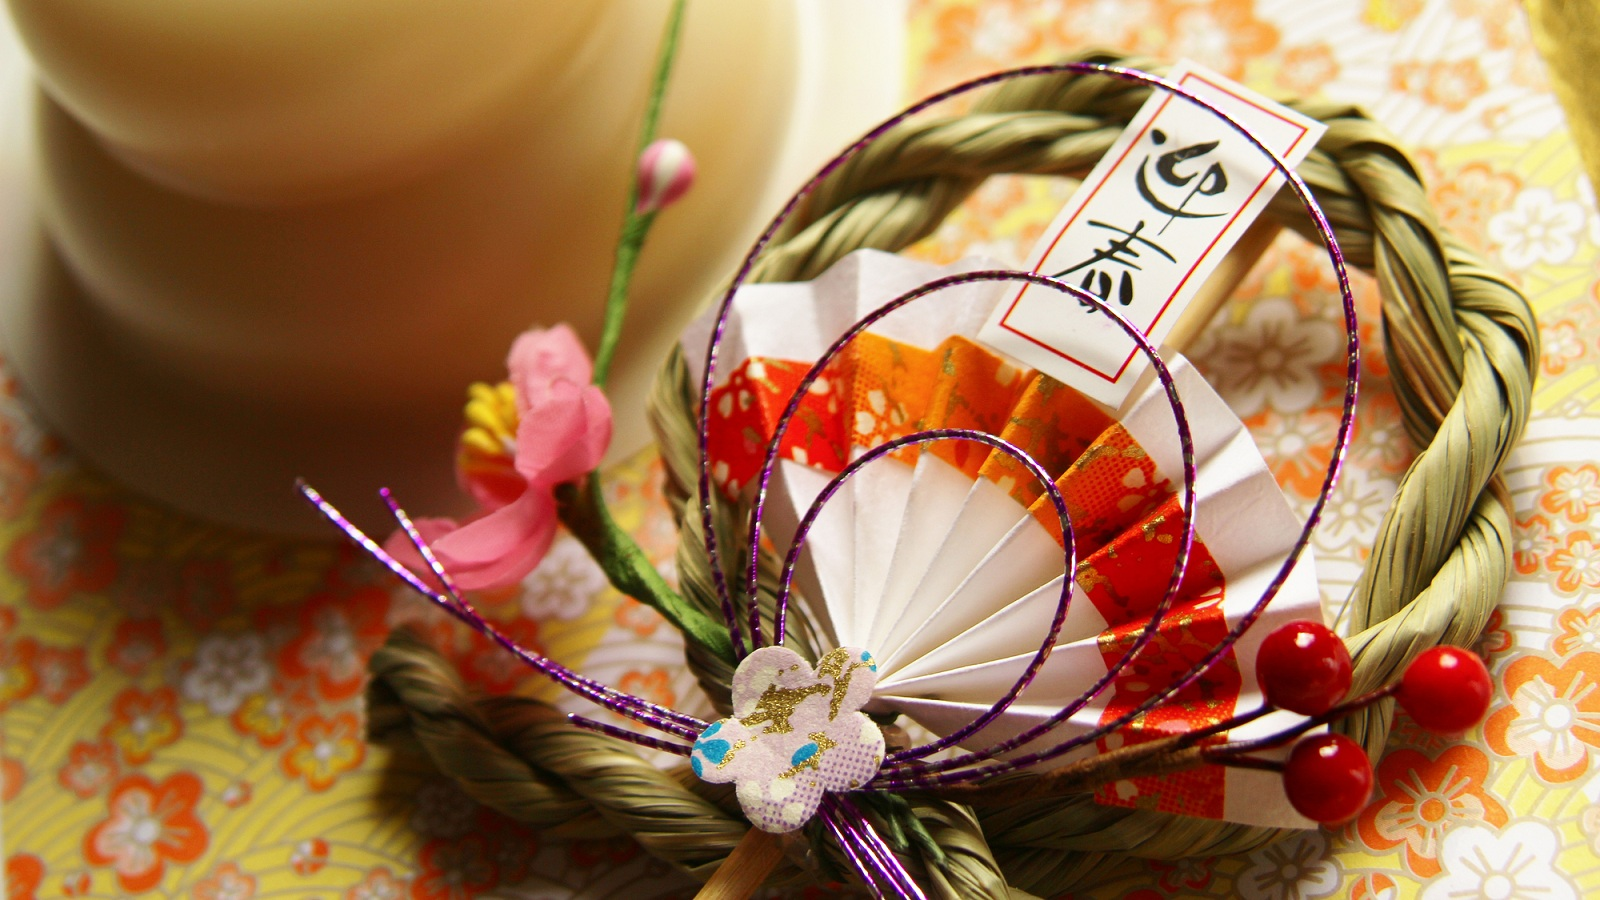
\includegraphics[width=0.8\linewidth]{images/11}
\end{center}
- Новий рік в Японії святкують не так, як у нас. В Україні — що веселіше, то вдаліший буде рік. Тут навпаки — що тихіше, то краще, — розповідає 35-річна Людмила Плис із Житомира. — Живих ялинок у Японії не бачила. Продають гілочки сосни. Їх ставлять у вази й прикрашають на Новий рік. Штучні ялинки теж бувають, але їх розбирають 26 грудня, після католицького Різдва. Я свою тримаю до 8 січня.

Людмила живе в японському місті Токай п'ять років. Вийшла заміж за старшого на 16 років Хіроюкі Кавагучі. Познайомилася з ним, коли їздила на заробітки в Японію 2008-го. За два роки він приїхав в Україну свататись. Після народження доньки подружжя переїхало на батьківщину Хіроюкі.

- У нашій сім'ї переважають японські традиції, але Різдво й Великдень святкуємо по-українськи. Має бути дідух, кутя і 12 страв.

У Японії Новий рік настає на 7 год. раніше, ніж в Україні.

- Стіл накриваю просто: фрукти, солодощі, шампанське. Чоловік майже одразу засинає, а я чекаю на наш Новий рік. Спілкуюся з рідними і друзями по скайпу. Вдень ідемо до свекрів.

- Проводжають рік з обов'язковою стравою тошікоші соба — локшиною з гречки. Символізує довге життя, здоров'я. Зранку починають їсти осечі рьорі — набір страв, складений у квадратну коробку. Обов'язкова — ікра оселедця, знак до поповнення в родині.

У Токаї Людмила — єдина слов'янка. Торік їй запропонували готувати українські страви для японців у ресторані ``Ада-Кода`` в сусідньому місті.

- Готую, як учила мама: борщ із пампушками, вареники з картоплею, холодець, салат із капусти й кропу, голубці з картопляним пюре, зелений борщ із чорним хлібом. В іншому ресторані ``Будинок томатів`` цілий грудень проводили місяць голубців. Японцям подобається наш чорний хліб з перекрученим салом і часником. Холодець нагадує їхню страву з морепродуктами — нікогорі.

Людмила спілкується з українцями з Токіо. Двічі на рік їздить у православну церкву. Машиною витрачає на дорогу 40 хв.

\vspace{1cm}

\NewsItem{Українські гердани та намиста популярні і в Японії}
%\NewsAuthor{}
\begin{center}
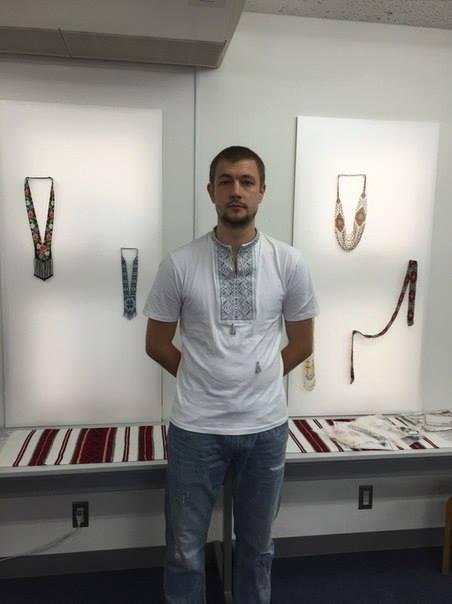
\includegraphics[width=0.8\linewidth]{images/8}
\end{center}
Киянин Максим Мамелін перетворив своє хоббі з бісероплетіння у професійну справу, приїхавши разом зі своєю дружиною в Японію влітку 2015 року. Почалося все ще 5 років тому, коли Макс захопився роботами своєї матері, почав плести сам, як хоббі, а сьогодні це стало професійним заняттям. З рук майстра виходять намиста, сережки, гердани, браслети та інши вироби з бісеру (бонсай, ялинкові прикраси та інше). Для популяризації бісероплетіння та своїх виробів Максим запрошує всіх приєднатись до групи facebook.com/groups/maksymsjewelry А в планах митця - проведення уроків та майстер класів для японських любителів ручного плетіння.

\end{multicols}

\newpage

\Category{Фотофакт}

\begin{center}
\NewsItem{4-й за рахунком Парад у Вишиванках пройшов в Токіо}	
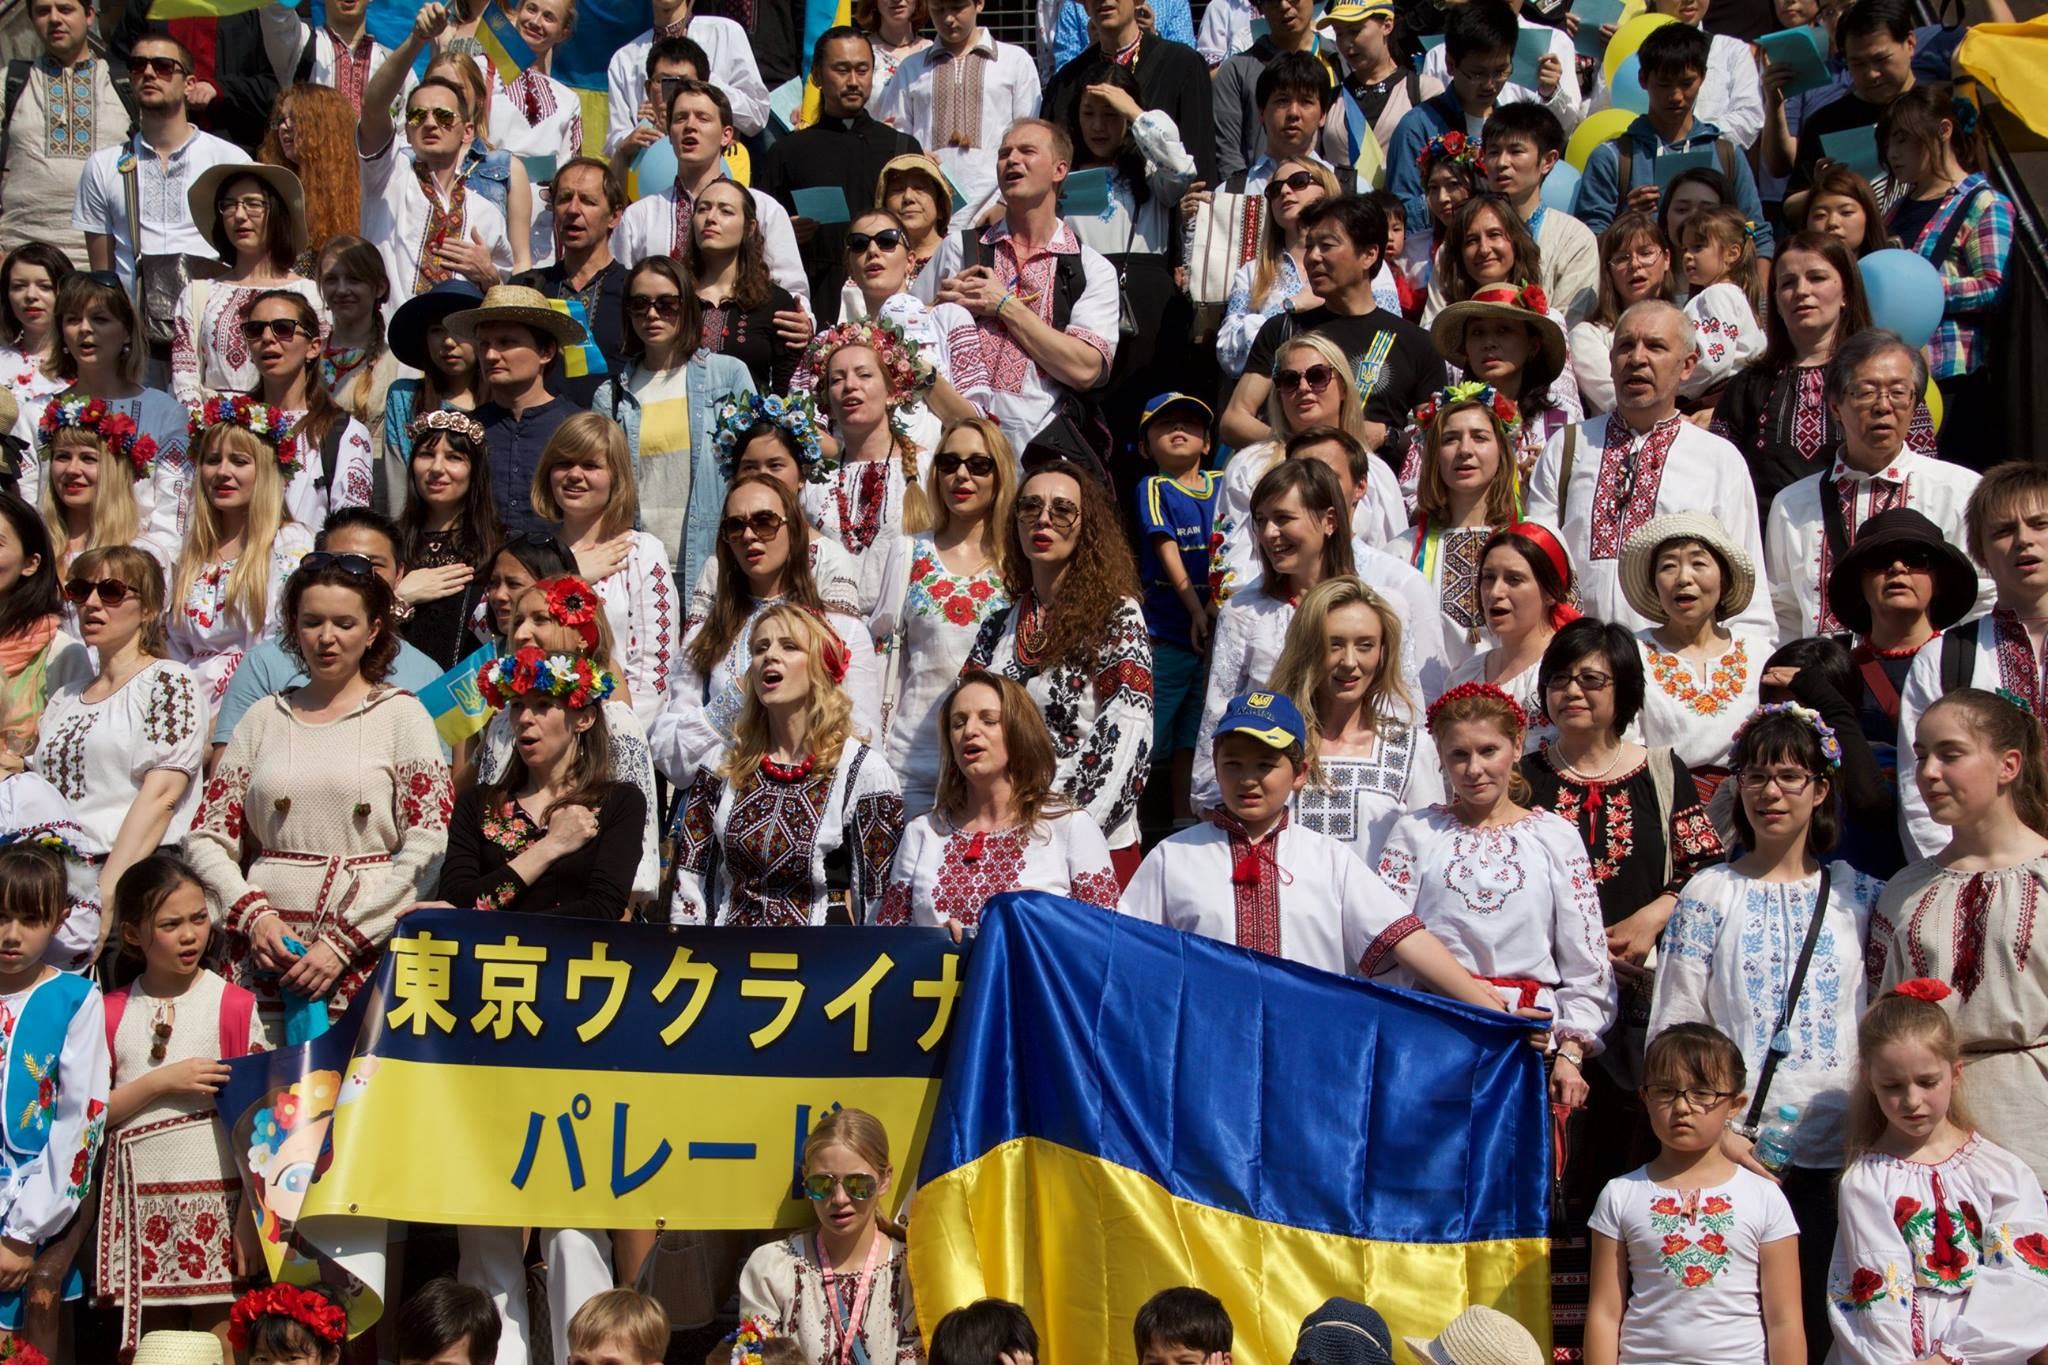
\includegraphics[width=0.6\textwidth]{images/14}
\end{center}

\SepRule	

\begin{center}
\NewsItem{Українська команда на щорічному фестивалі ''Серце до серця 2016'' в місті Токай}
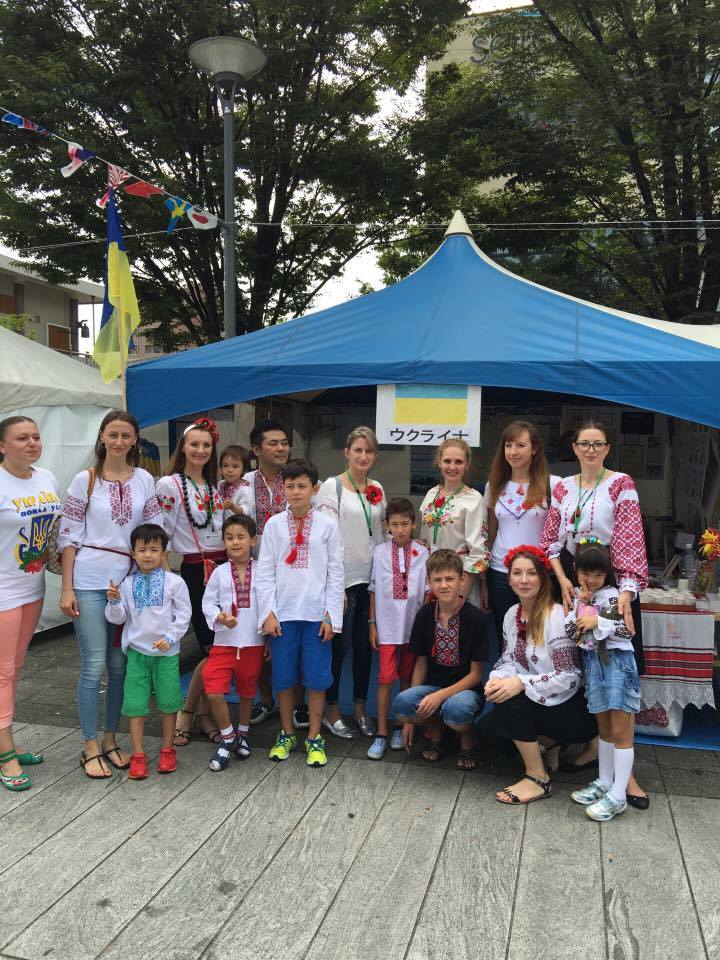
\includegraphics[width=0.6\textwidth]{images/17}
\end{center}

\newpage

\begin{center}
\NewsItem{День Святого Миколая у Школі ``Джерельце``}	
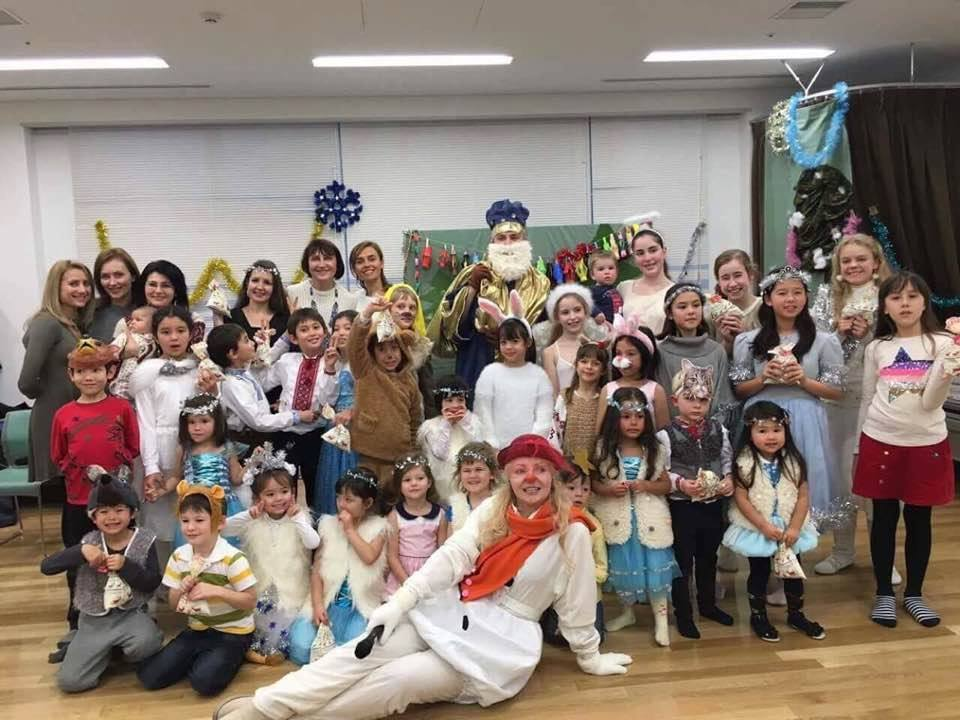
\includegraphics[width=0.9\textwidth]{images/20}
\end{center}

\SepRule	

\begin{center}
\NewsItem{Виступ оперної співачки Оксани Степанюк на фестивалі ''День України''}
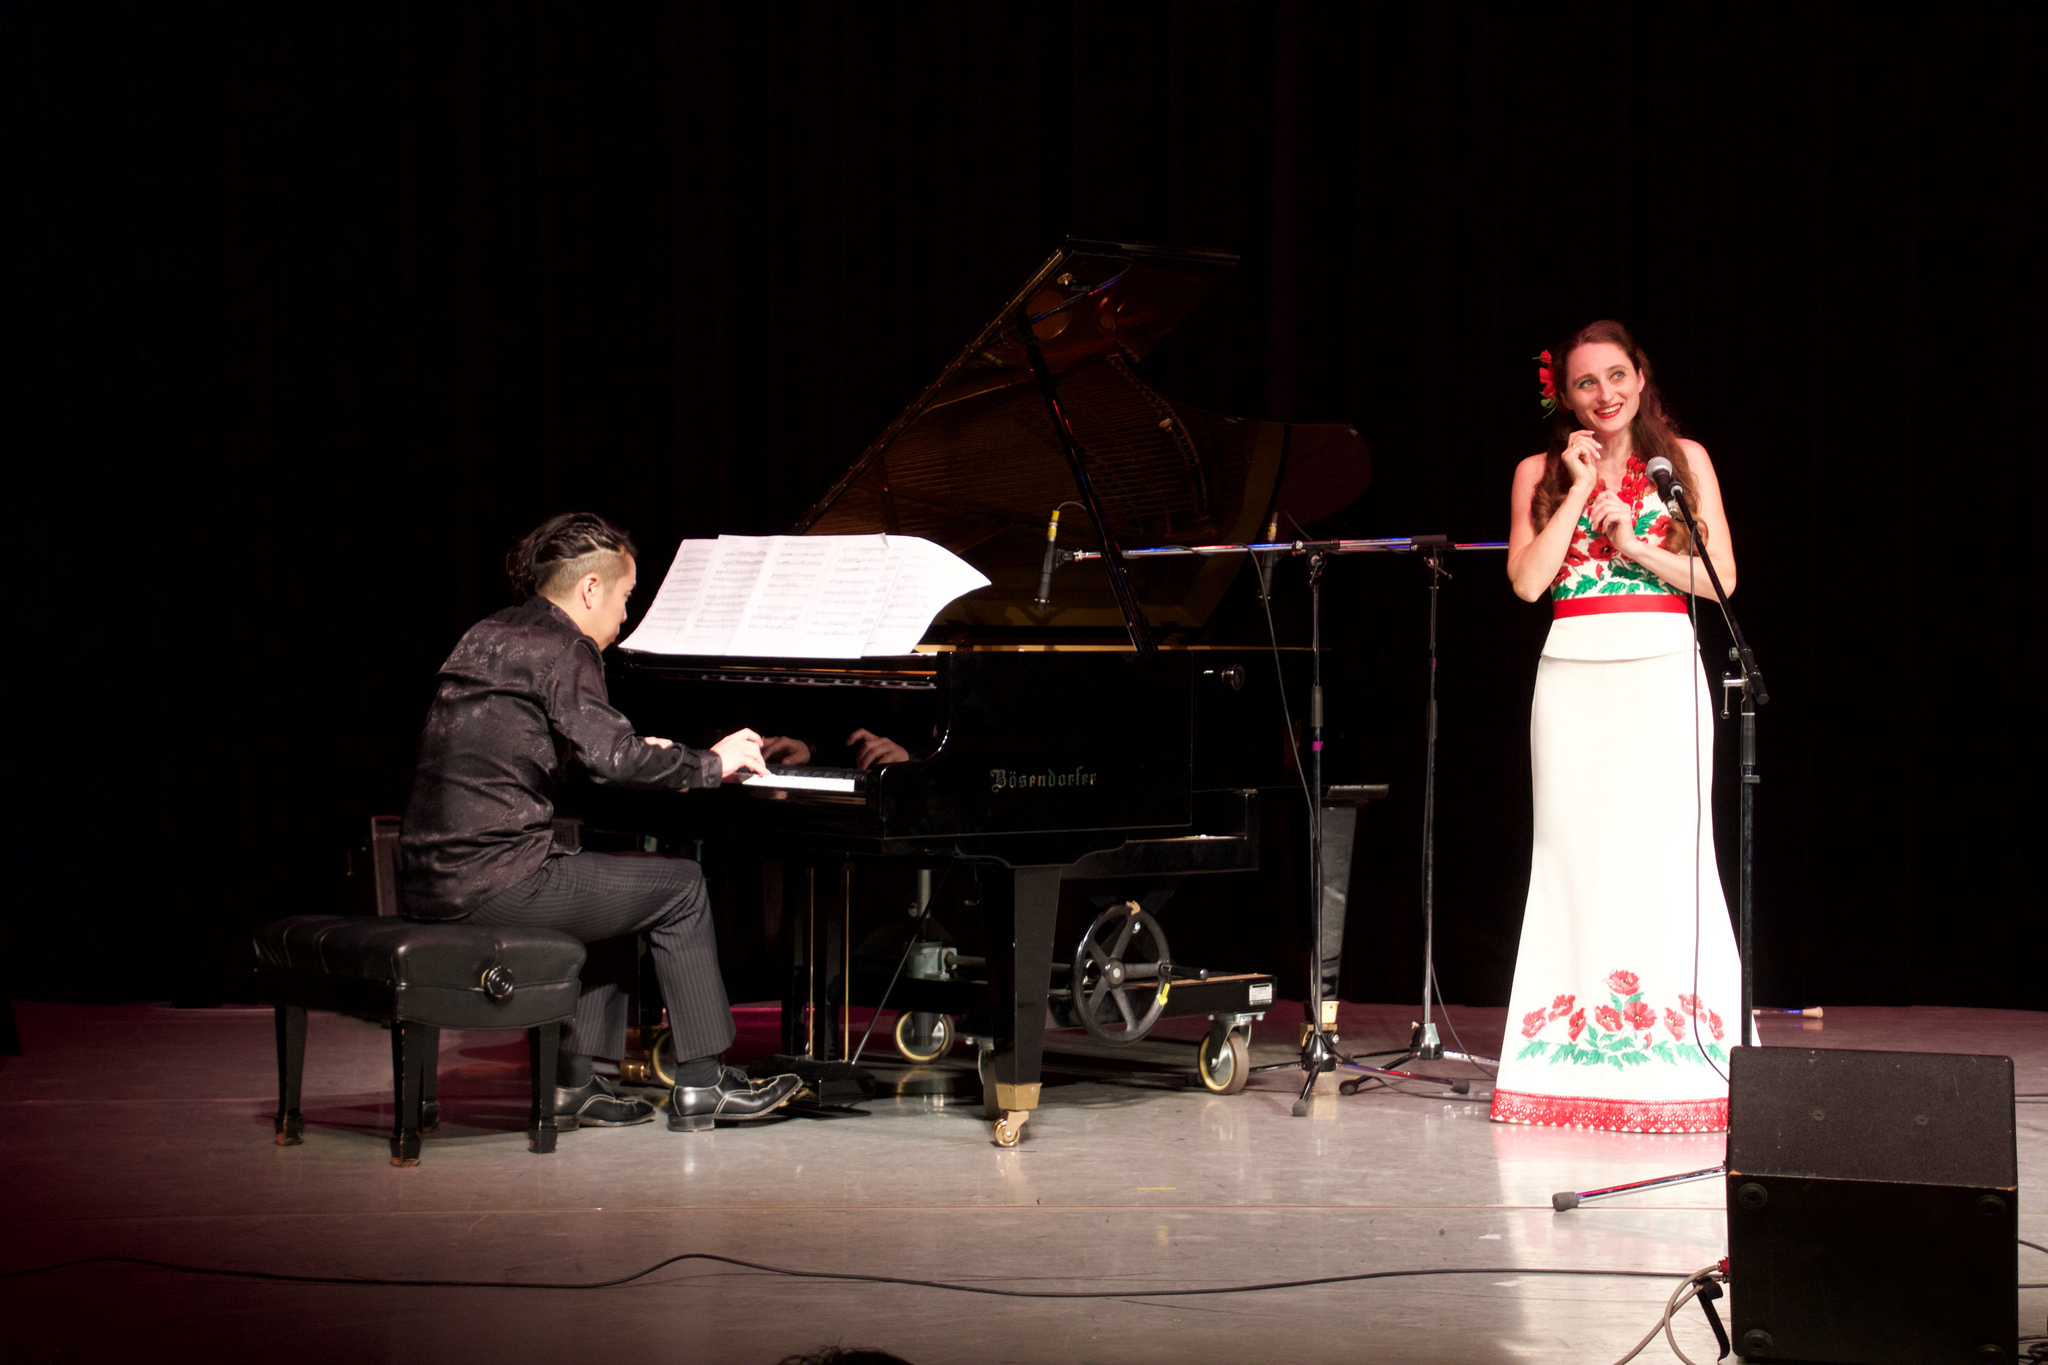
\includegraphics[width=0.9\textwidth]{images/21}
\end{center}

\newpage

\begin{center}
\NewsItem{Виступ дітей з української недільної школи ``Джерельце``}	
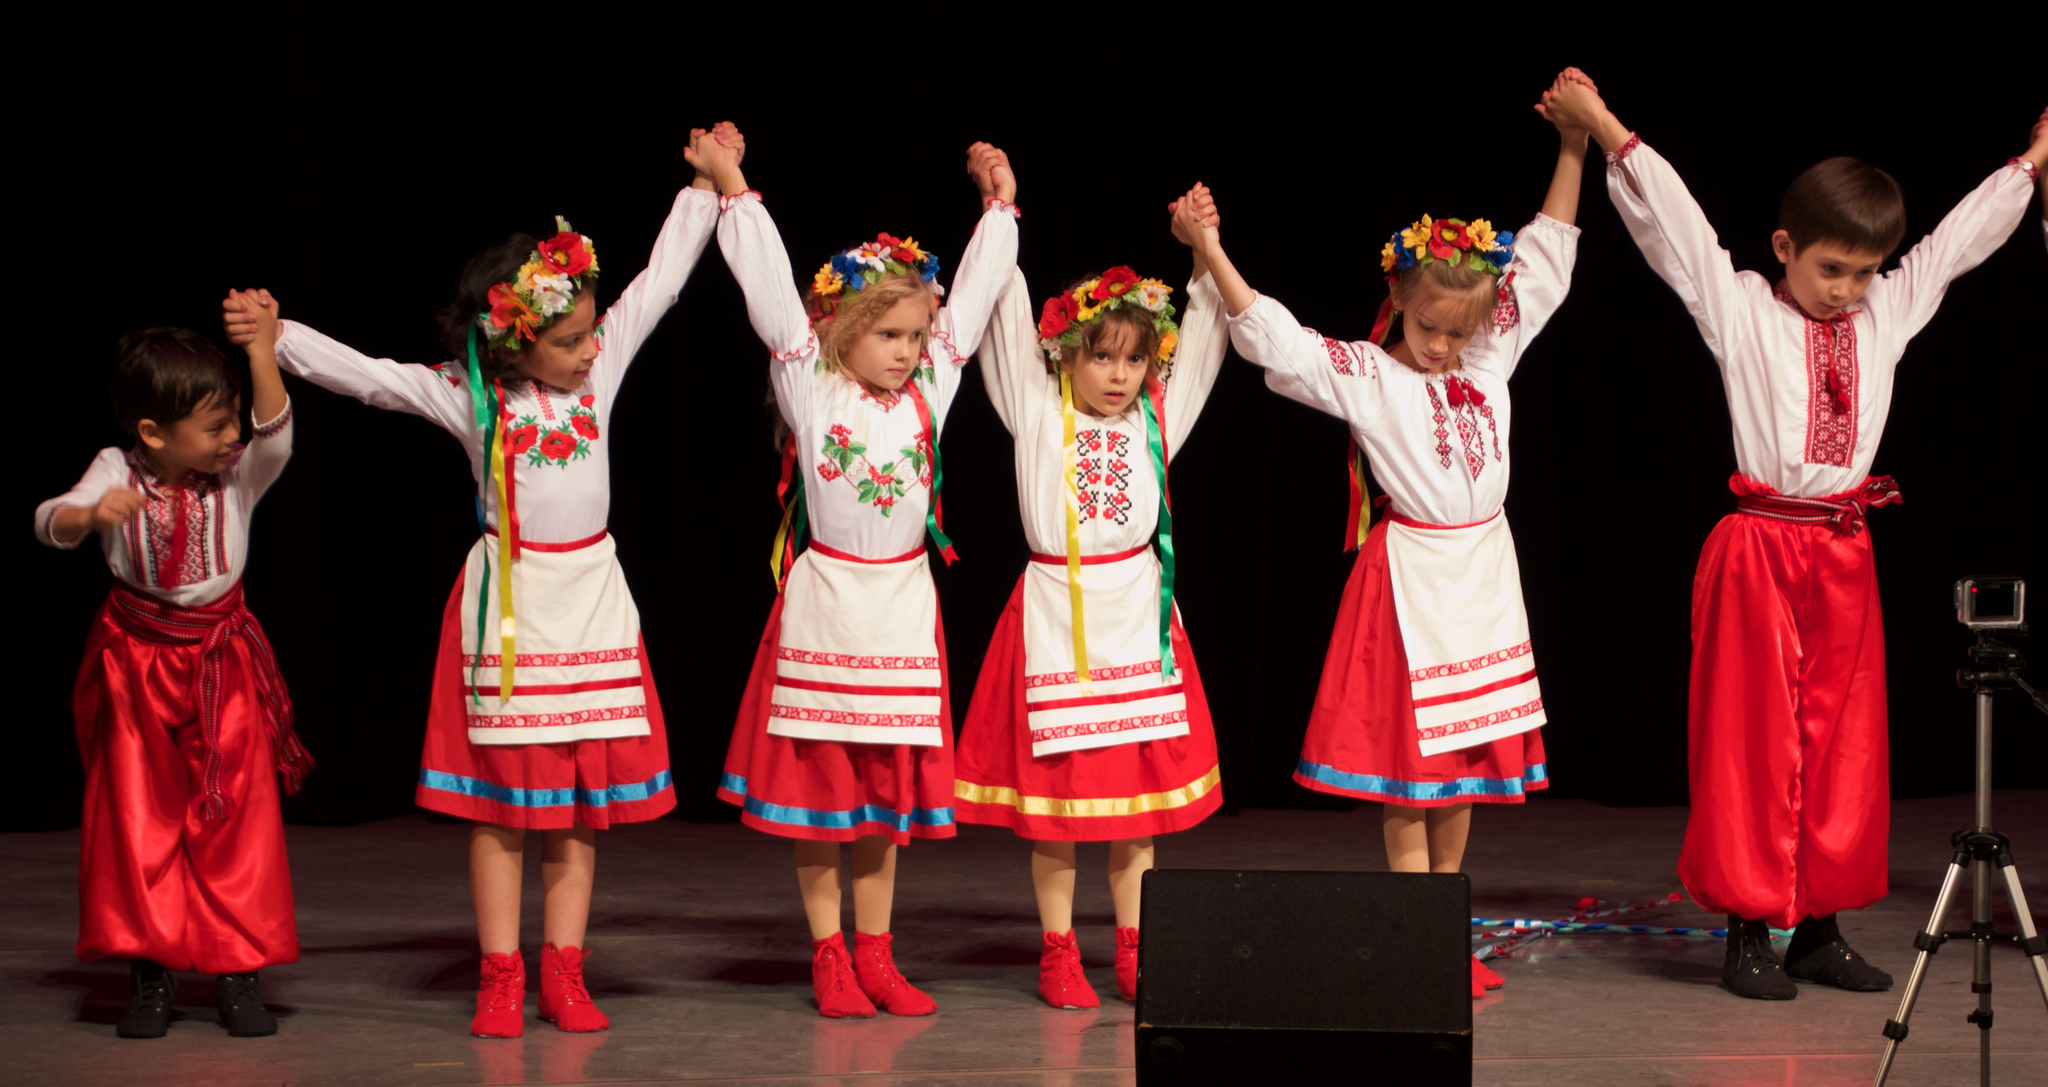
\includegraphics[width=0.9\textwidth]{images/22}
\end{center}

\SepRule	

\begin{center}
\NewsItem{Хореографічна композиція ``Заплуталась`` (Юлія Сидоренко та Марина Амаурі)}
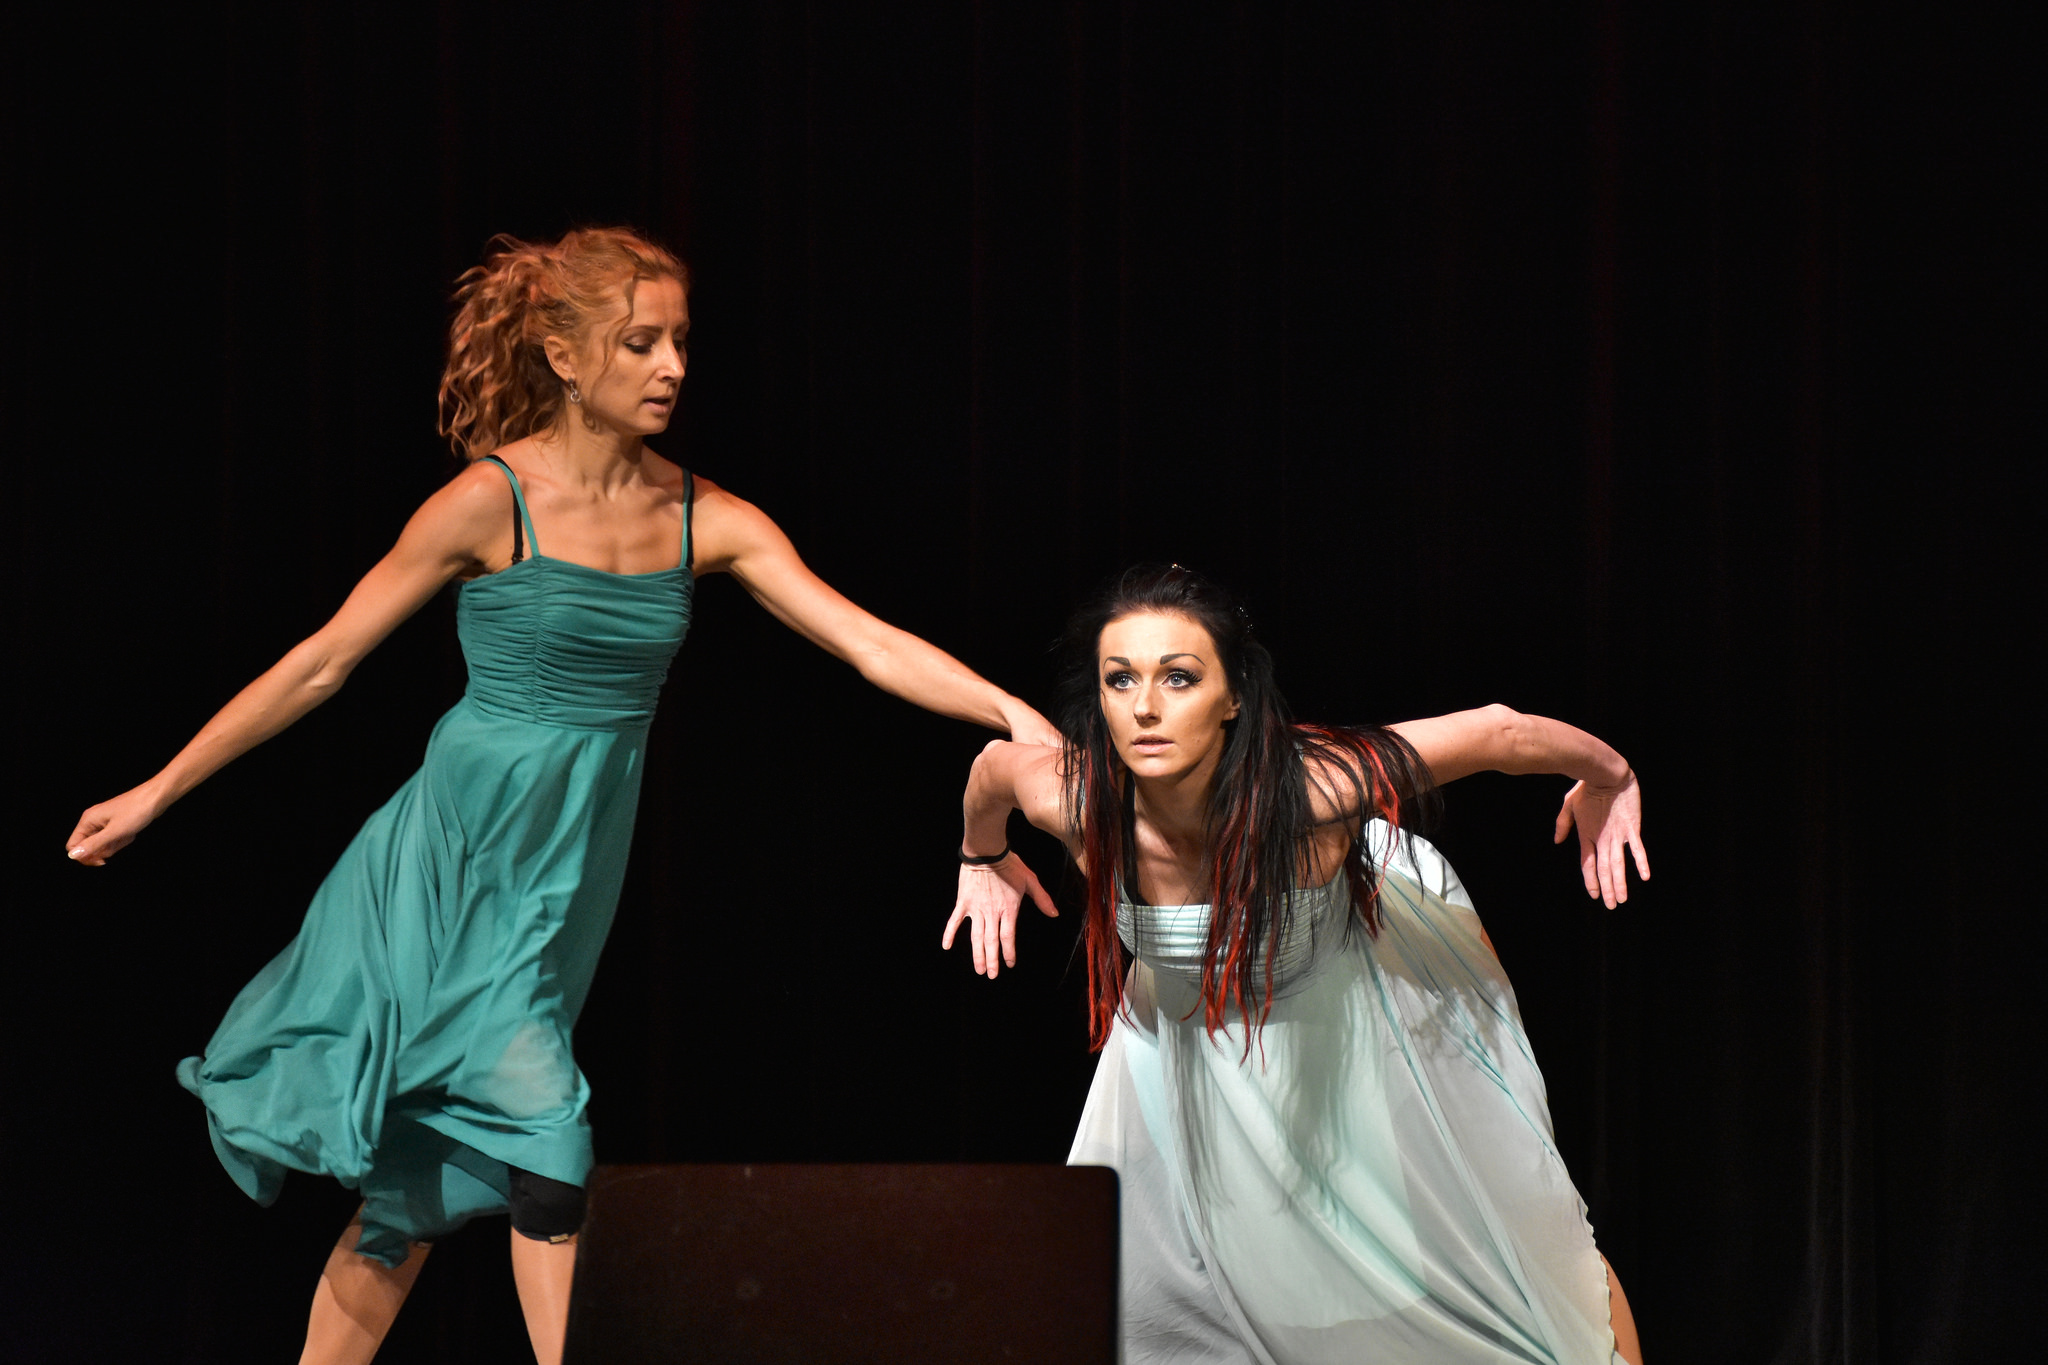
\includegraphics[width=0.9\textwidth]{images/23}
\end{center}

\newpage

\begin{center}
\NewsItem{Джазовий концерт на фестивалі ``День України``}	
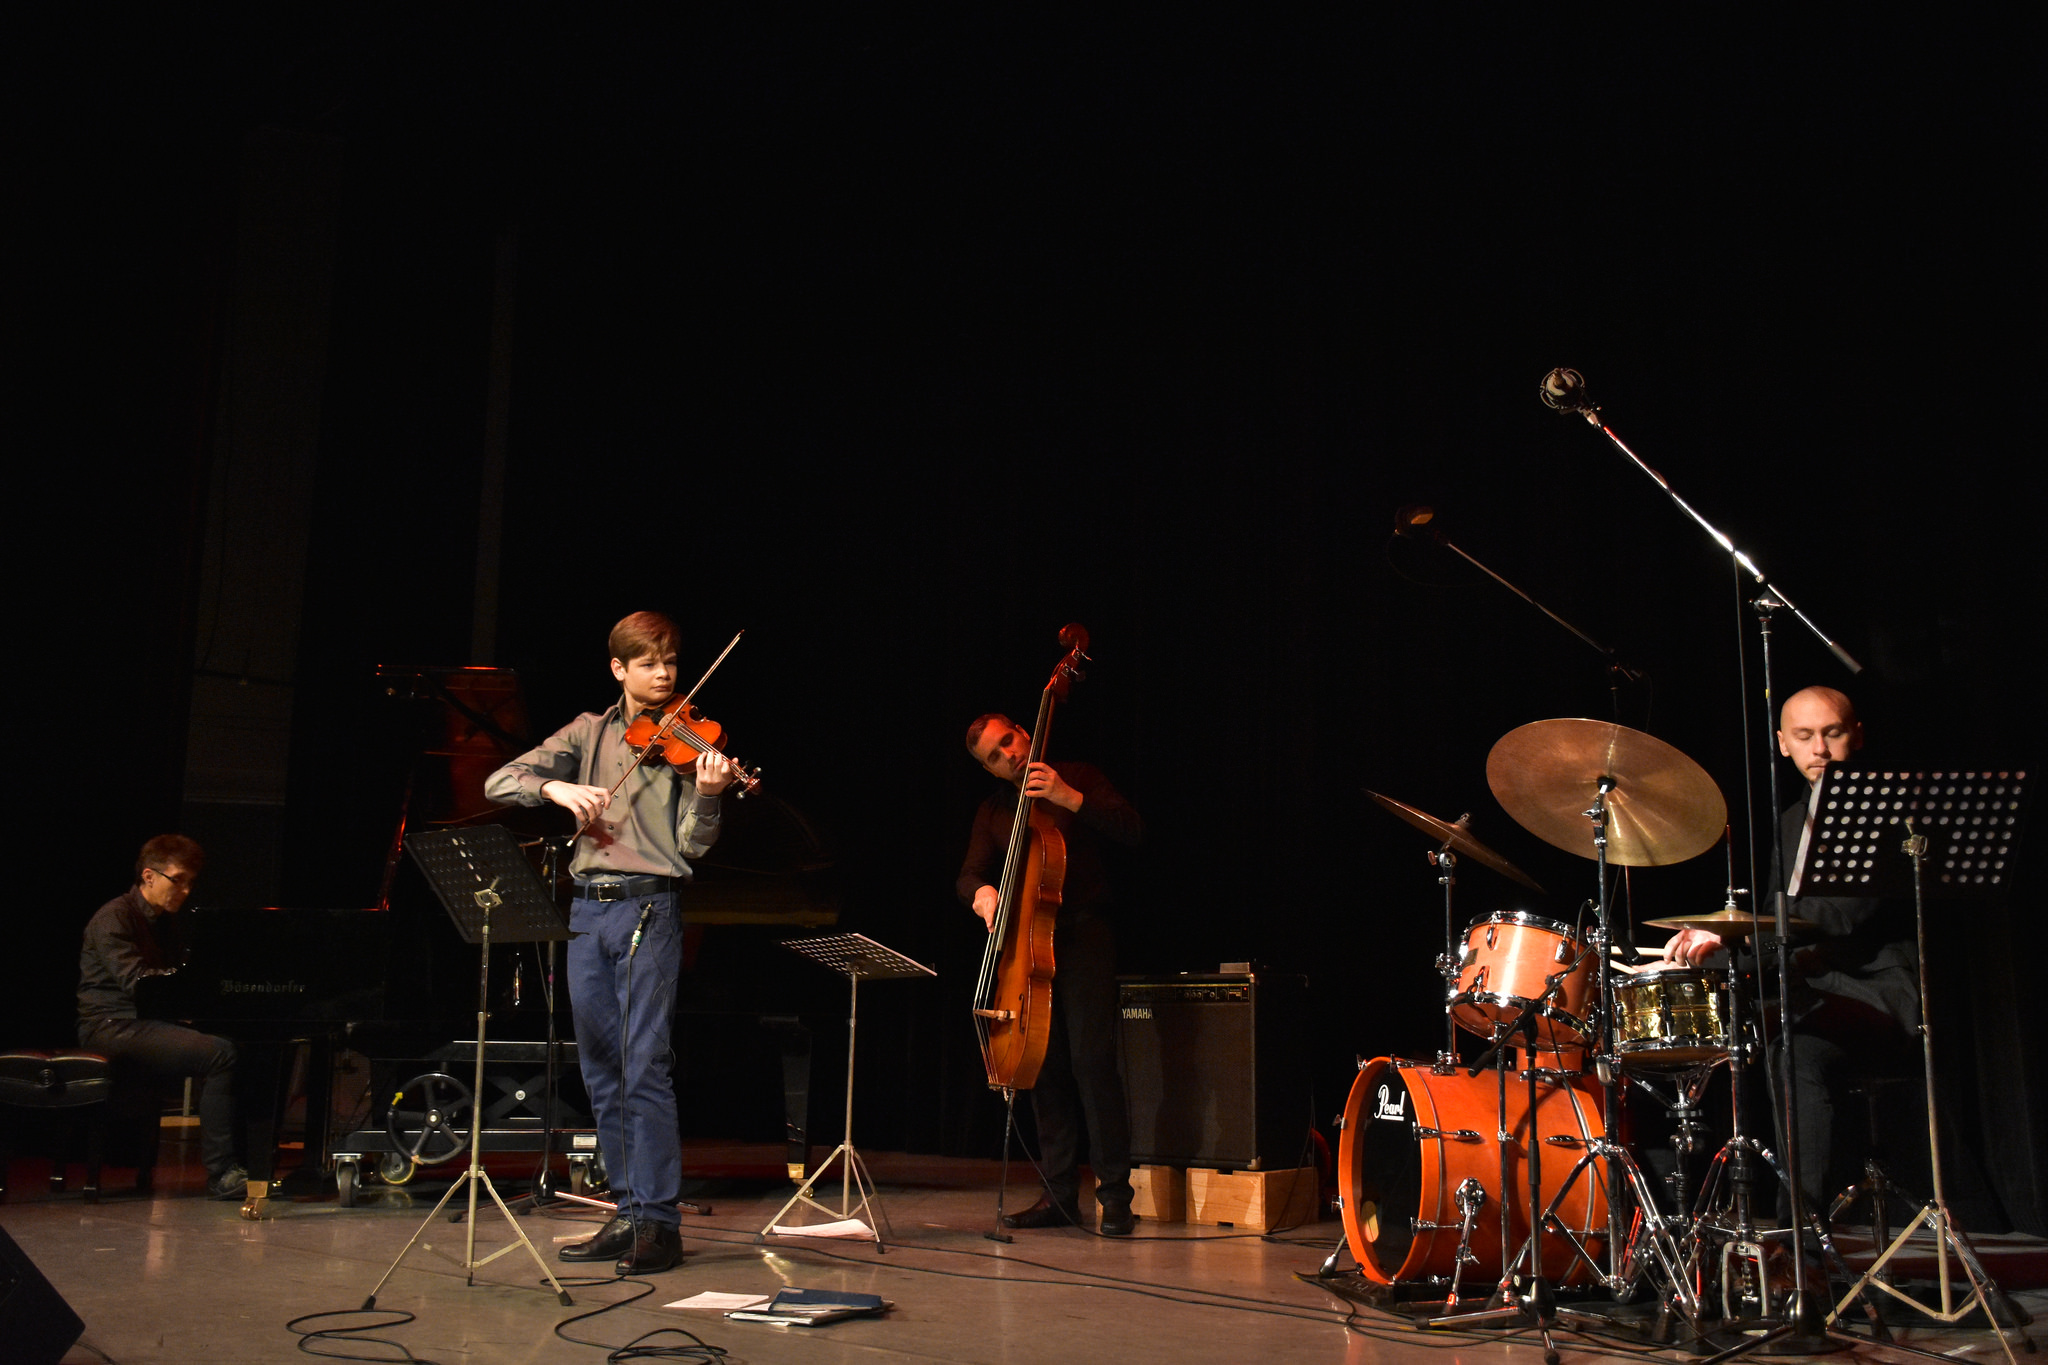
\includegraphics[width=0.9\textwidth]{images/24}
\end{center}

\SepRule	

\begin{center}
\NewsItem{Українські прикраси з бісеру від майстра Максима Мамеліна}
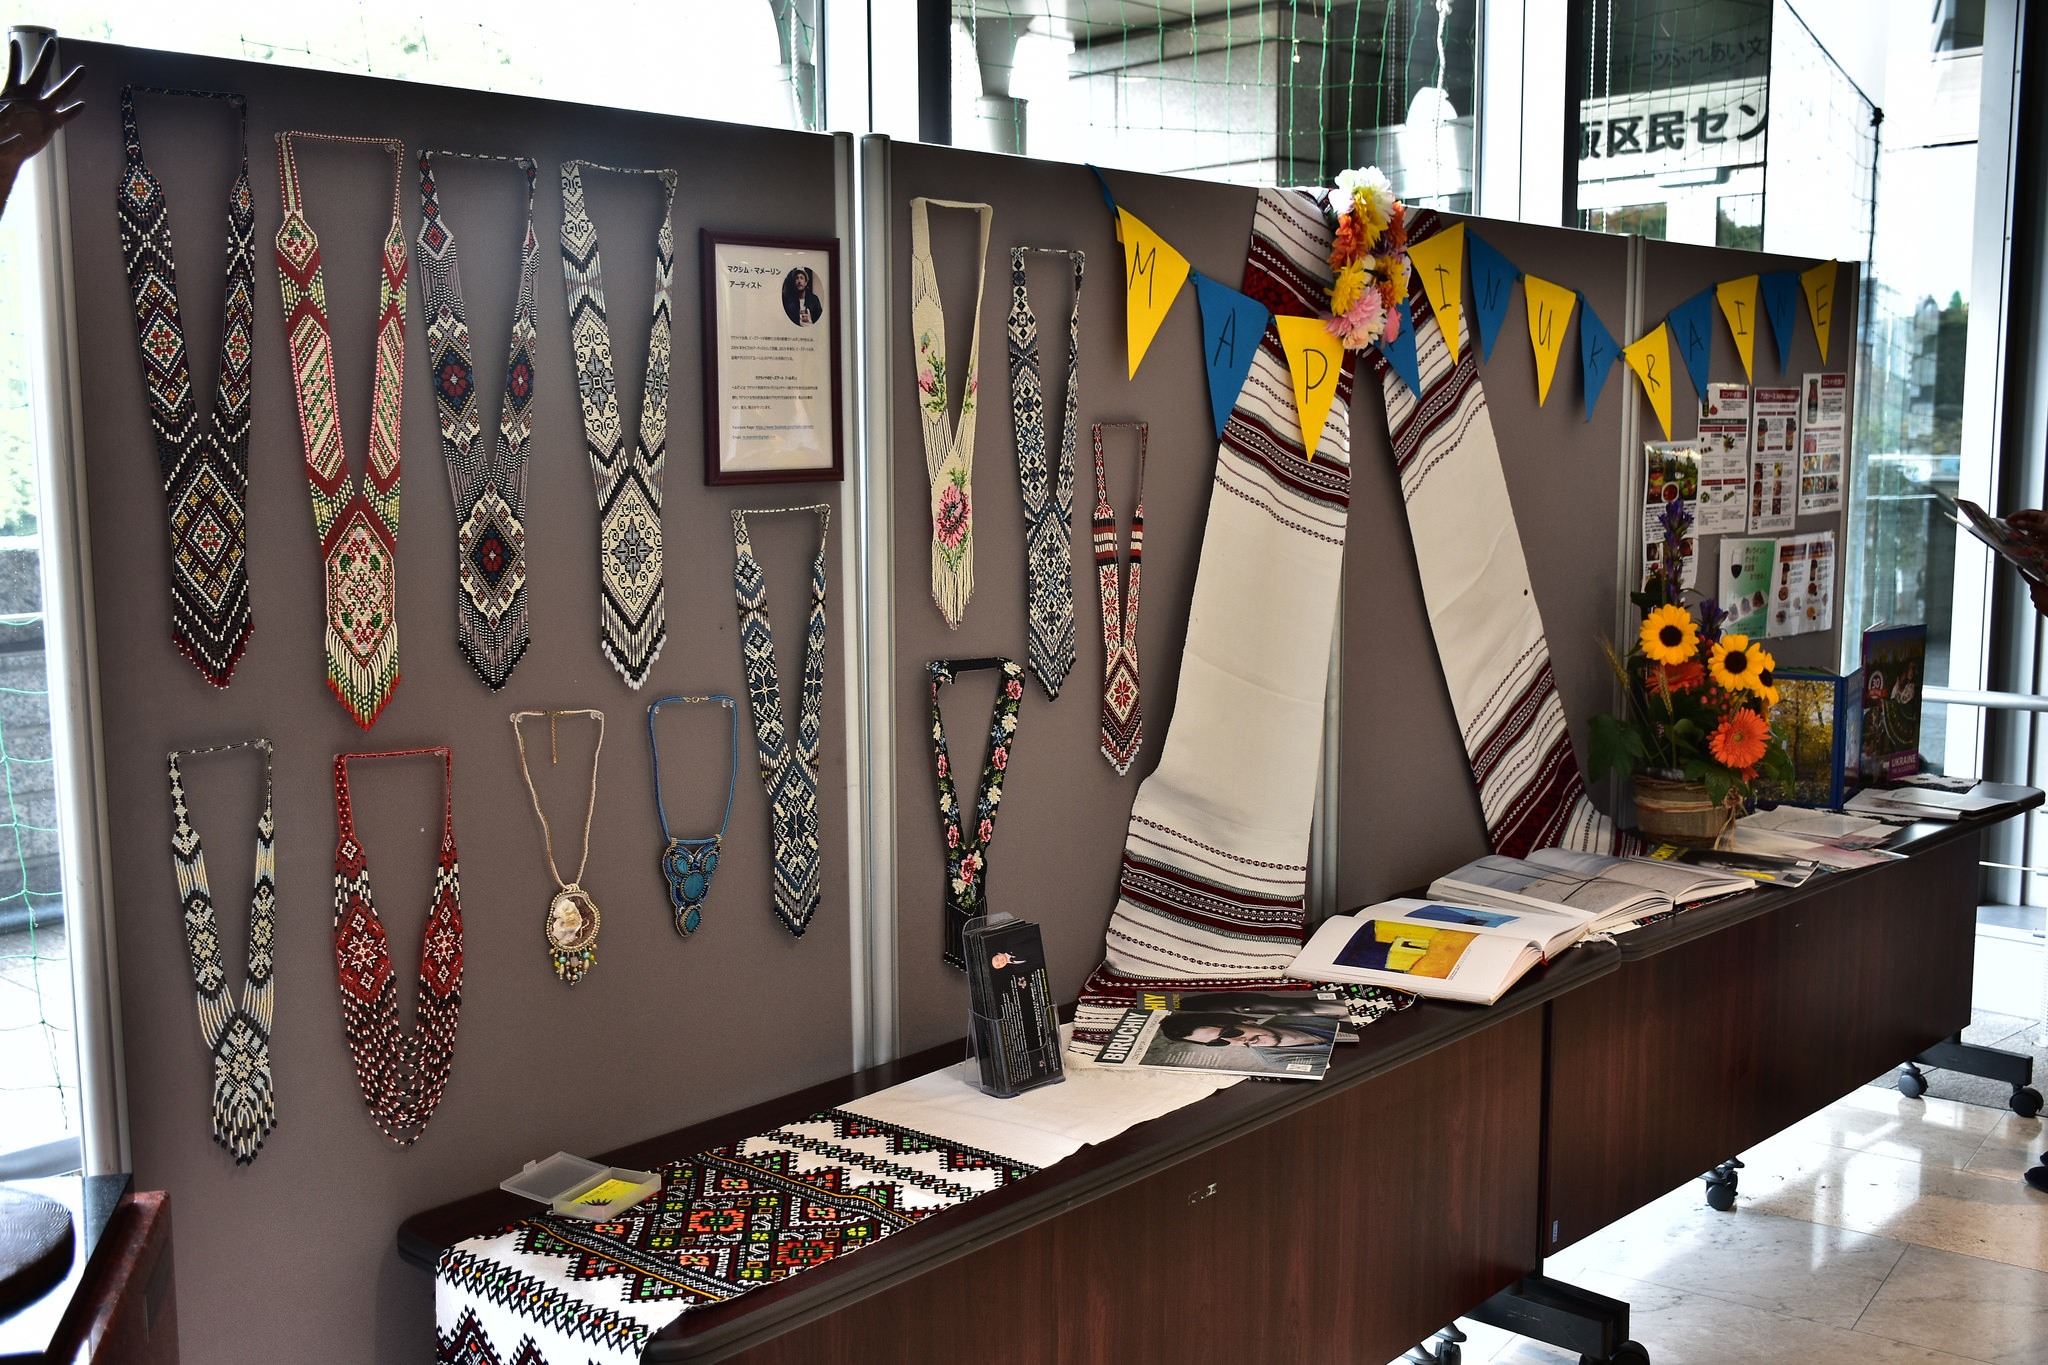
\includegraphics[width=0.9\textwidth]{images/26}
\end{center}

\newpage

\begin{center}
\NewsItem{Японський музичний інструмент кокю (В'ячеслав Онищенко)}
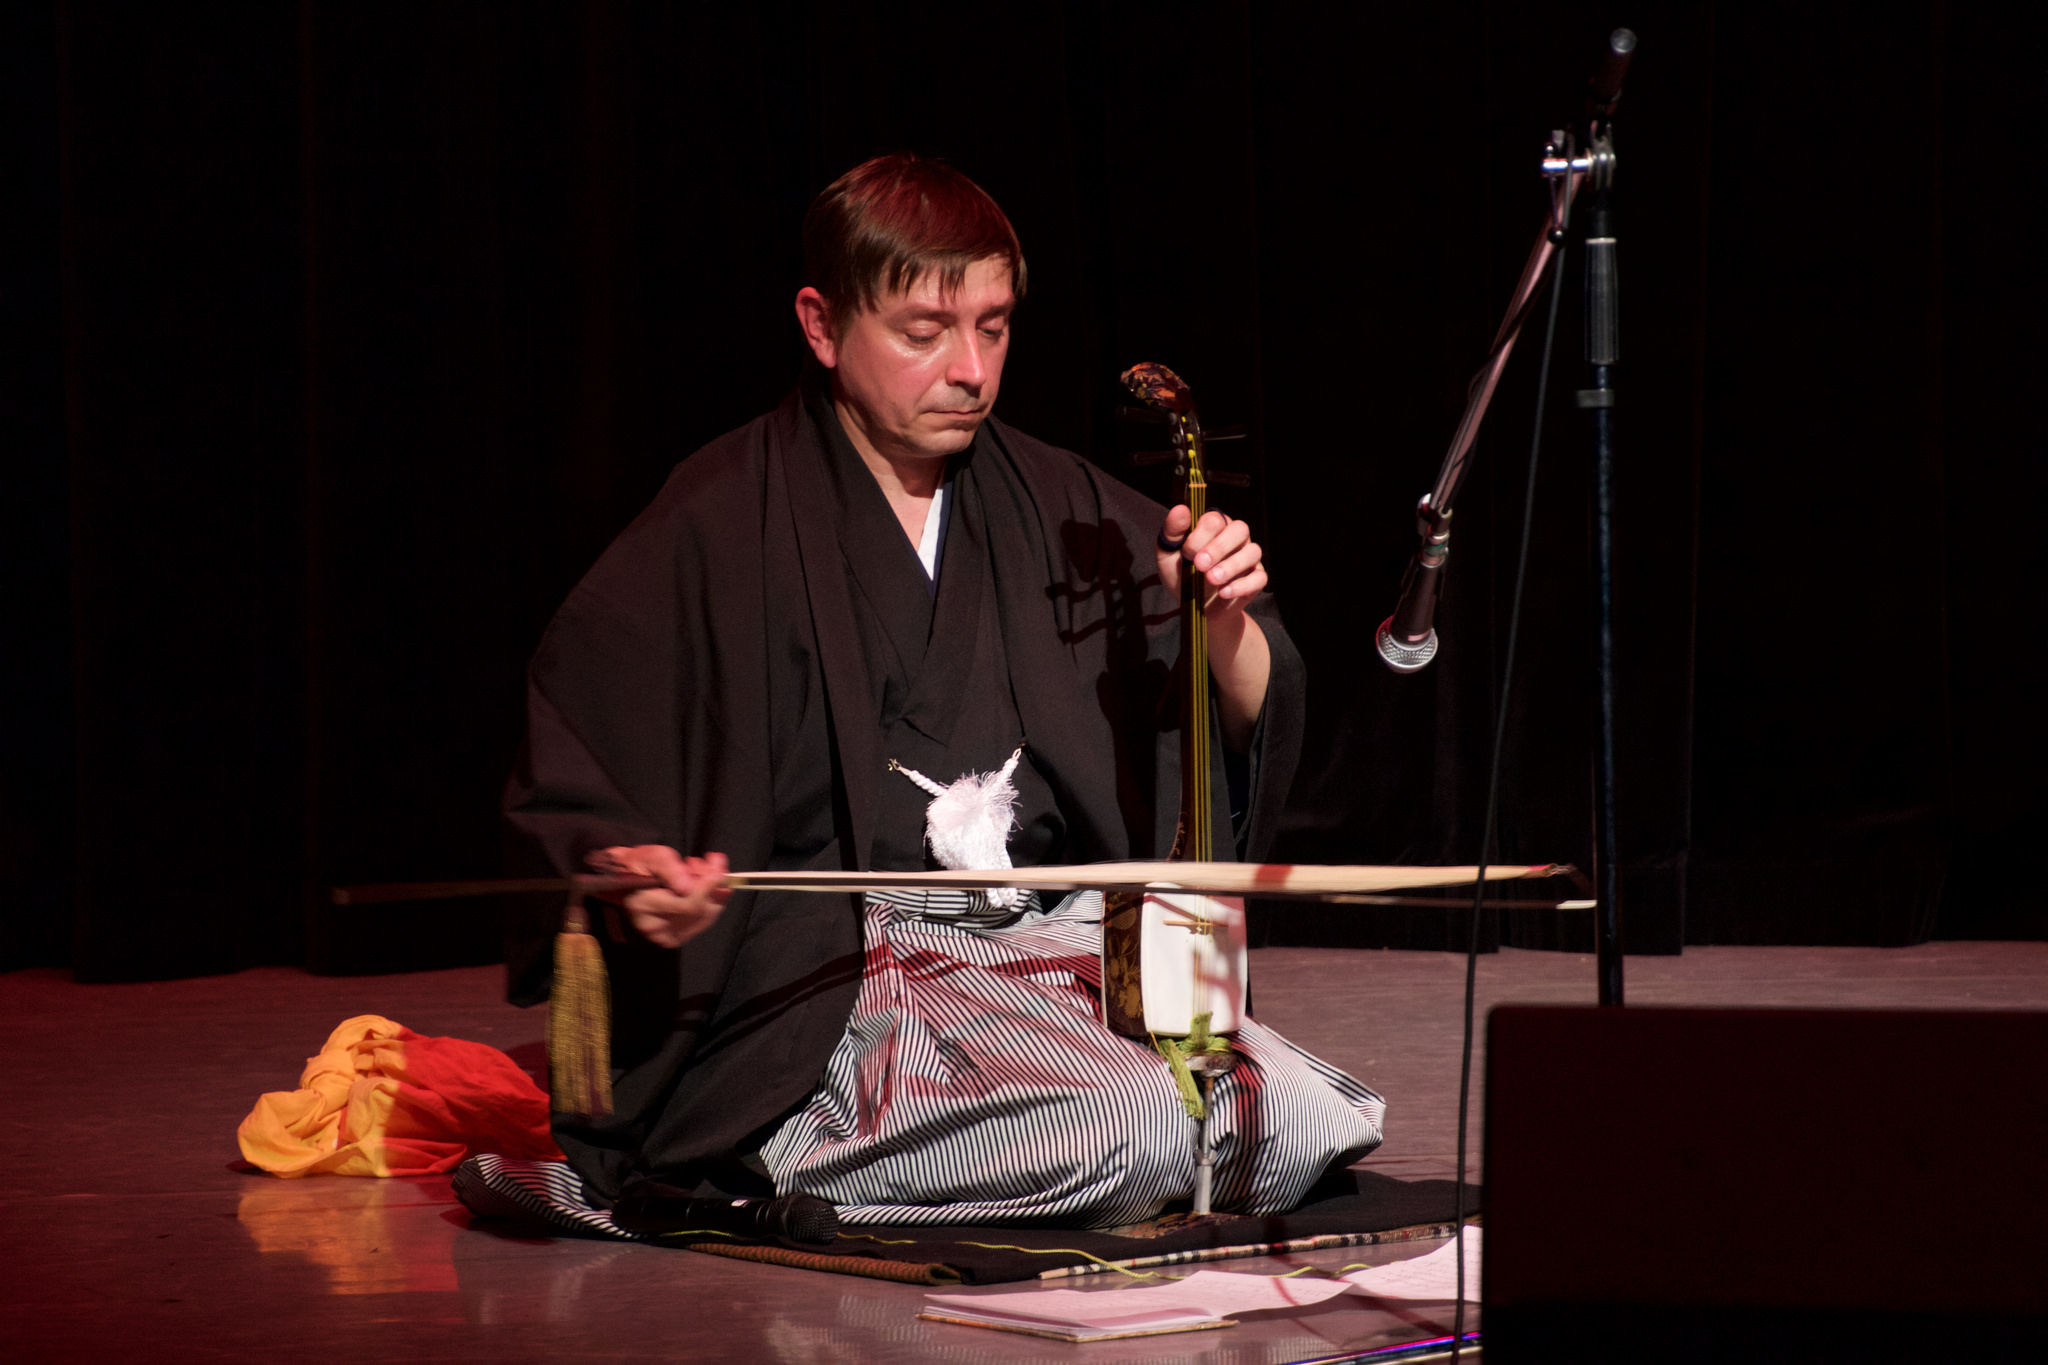
\includegraphics[width=0.9\textwidth]{images/27}
\end{center}

\SepRule	

\begin{center}
\NewsItem{Gypsy Skirt Dance від хореографа Elina Star}	
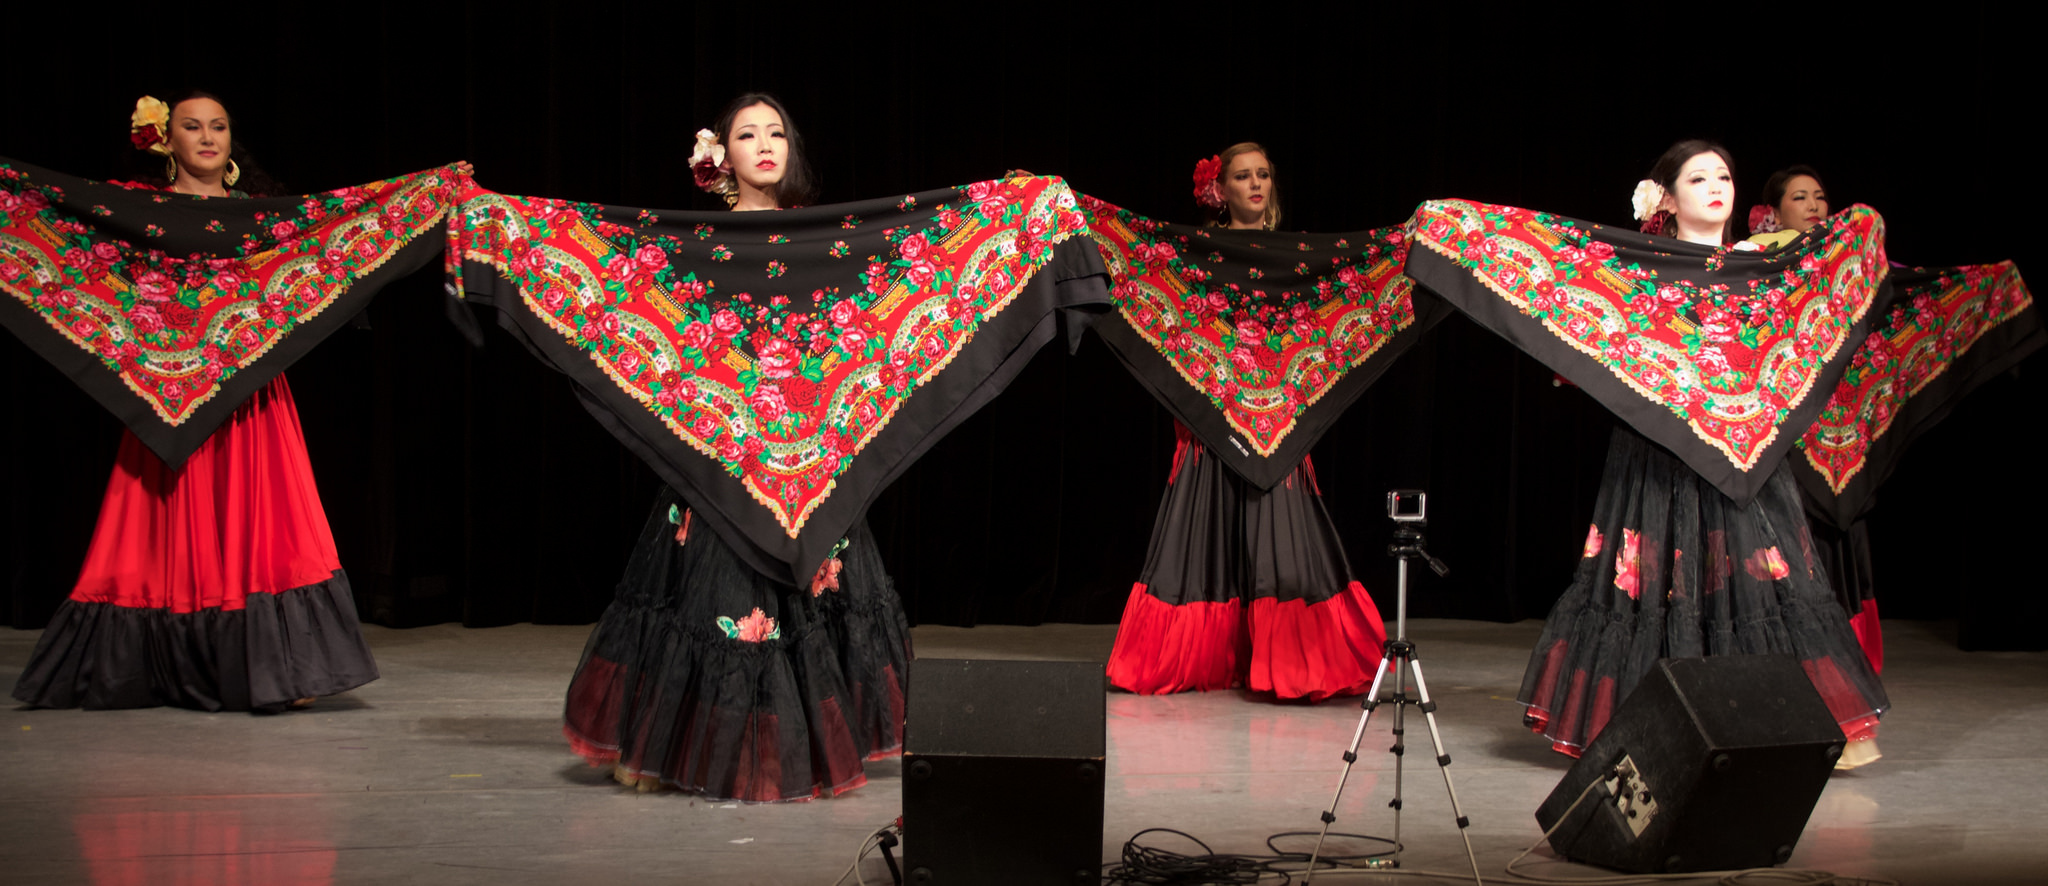
\includegraphics[width=0.9\textwidth]{images/25}
\end{center}

\newpage

\begin{center}

\includegraphics[width=0.8\linewidth]{images/tryzub}
\SepRule			
Цей випуск Часопису присвячується 25-й річниці з Дня Проголошення Незалежності України та Героям України всіх часів, які поклали своє життя за Її волю та незалежність.
\end{center}

\end{document}
